%  LaTeX support: latex@mdpi.com 
%  In case you need support, please attach all files that are necessary for compiling as well as the log file, and specify the details of your LaTeX setup (which operating system and LaTeX version / tools you are using).

% You need to save the "mdpi.cls" and "mdpi.bst" files into the same folder as this template file.

%=================================================================
\documentclass[energies,article,submit,moreauthors,latex,10pt,a4paper]{mdpi} 
%
%--------------------
% Class Options:
%--------------------
% journal
%----------
% Choose between the following MDPI journals:
% actuators, addictions, admsci, aerospace, agriculture, agronomy, algorithms, animals, antibiotics, antibodies, antioxidants, applsci, arts, atmosphere, atoms, axioms, batteries, bdcc, behavsci, beverages, bioengineering, biology, biomedicines, biomimetics, biomolecules, biosensors, brainsci, buildings, carbon, cancers, catalysts, cells, challenges, chemengineering, chemosensors, children, chromatography, climate, coatings, colloids, computation, computers, condensedmatter, cosmetics, cryptography, crystals, cybersecurity, data, dentistry, designs, diagnostics, diseases, diversity, econometrics, economies, education, electrochemistry, electronics, energies, entropy, environments, epigenomes, fermentation, fibers, fishes, fluids, foods, forests, fractalfract, futureinternet, galaxies, games, gastrointestdisord, gels, genealogy, genes, geosciences, geriatrics, healthcare, highthroughput, horticulturae, humanities, hydrology, informatics, information, infrastructures, inorganics, insects, instruments, ijerph, ijfs, ijms, ijgi, ijtpp, inventions, jcdd, jcm, jcs, jdb, jfb, jfmk, jimaging, jof, jintelligence, jlpea, jmmp, jmse, jpm, jrfm, jsan, land, languages, laws, life, literature, logistics, lubricants, machines, magnetochemistry, make, marinedrugs, materials, mathematics, mca, mti, medsci, medicines, membranes, metabolites, metals, microarrays, micromachines, microorganisms, minerals, molbank, molecules, mps, nanomaterials, ncrna, neonatalscreening, nitrogen, nutrients, ohbm, particles, pathogens, pharmaceuticals, pharmaceutics, pharmacy, philosophies, photonics, plants, plasma, polymers, proceedings, processes, proteomes, publications, quaternary, qubs, recycling, religions, remotesensing, resources, risks, robotics, safety, scipharm, sensors, separations, sexes, sinusitis, socsci, societies, soils, sports, standards, surgeries, sustainability, symmetry, systems, technologies, toxics, toxins, tropicalmed, universe, urbansci, vaccines, vetsci, viruses, vision, water, wem
%---------
% article
%---------
% The default type of manuscript is article, but can be replaced by: 
% addendum, article, benchmark, book, bookreview, briefreport, casereport, changes, comment, commentary, communication, conceptpaper, correction, conferenceproceedings, conferencereport, expressionofconcern, meetingreport, creative, datadescriptor, discussion, editorial, essay, erratum, hypothesis, interestingimages, letter, newbookreceived, opinion, obituary, projectreport, reply, reprint, retraction, review, perspective, preprints, protocol, shortnote, supfile, technicalnote, viewpoint
% supfile = supplementary materials
% protocol: If you are preparing a "Protocol" paper, please refer to http://www.mdpi.com/journal/mps/instructions for details on its expected structure and content.
%----------
% submit
%----------
% The class option "submit" will be changed to "accept" by the Editorial Office when the paper is accepted. This will only make changes to the frontpage (e.g. the logo of the journal will get visible), the headings, and the copyright information. Also, line numbering will be removed. Journal info and pagination for accepted papers will also be assigned by the Editorial Office.
%------------------
% moreauthors
%------------------
% If there is only one author the class option oneauthor should be used. Otherwise use the class option moreauthors.
%---------
% pdftex
%---------
% The option pdftex is for use with pdfLaTeX. If eps figure are used, remove the option pdftex and use LaTeX and dvi2pdf.

%%%%%%%%%%%%%%%%%%%%%%%%%%%%%%%%%%%%%%%%
\usepackage{tabularx}
\usepackage{mathtools}
\usepackage{mathrsfs}
\usepackage{amsmath}
%\usepackage[short]{optidef}
\usepackage{xcolor}
\usepackage{amsfonts}

% Colors
%---------------------------------------------------------------------------------
\definecolor{C1}{RGB}{31,119,180}
\definecolor{C2}{RGB}{255,127,14}
\definecolor{C3}{RGB}{44,160,44}
\definecolor{C4}{RGB}{214,39,40}

\newcommand{\revision}[1]{{\color{red} #1}}

% Some  auxiliary commands for ease of mathematics notations
%---------------------------------------------------------------------------------
% Derivatives and differentials
\newcommand{\ds}{~\text{d}\boldsymbol{s}}
\newcommand{\dzeta}{~\text{d}\boldsymbol{\zeta}}
\newcommand{\pder}[2]{\frac{\partial #1}{\partial #2}}
\newcommand{\bs}[1]{\boldsymbol{#1}}
\newcommand{\dx}{\text{d}\boldsymbol{x}}
\newcommand{\dt}{\text{d}t}
\newcommand{\ddt}[1]{\frac{\text{d} #1}{\text{d} t}}
% Integrals
\newcommand{\stint}{\int_{0}^{T} \int_{\Omega}}
\newcommand{\sint}{\int_{\Omega}}
\newcommand{\Tint}{\int_{0}^{T}}
\newcommand{\tint}{\int_{0}^{t}}
% Filtered variables
\newcommand{\utilde}{\widetilde{\bs{u}}}
\newcommand{\ptilde}{\widetilde{p}}
\newcommand{\ctnhat}[1]{\widehat{C}_{T,#1}'}
\newcommand{\ctihat}{\widehat{C}_{T,i}'}
\newcommand{\cthat}{\widehat{C}_T'}
% Other symbols
\newcommand{\ctmax}{C_{T,\text{max}}'}
\newcommand{\cti}{C_{T,i}'}
\newcommand{\ctn}[1]{C_{T,#1}'}
\newcommand{\R}{\mathscr{R}}
\newcommand{\J}{\mathscr{J}}
\newcommand{\Jtilde}{\tilde{\mathscr{J}}}
\newcommand{\Jgrad}{\nabla \Jtilde}
\newcommand{\Lagr}{\mathscr{L}}
\newcommand{\eperp}{\bs{e}_\perp}
\newcommand{\eperpi}{\bs{e}_{\perp,i}}
\newcommand{\etransi}{\bs{e}_{\parallel,i}}
\newcommand{\ex}{\bs{e}_x}
\newcommand{\ey}{\bs{e}_y}
\newcommand{\ez}{\bs{e}_z}
\newcommand{\eperpn}[1]{\bs{e}_{\perp,#1}}
\newcommand{\vi}{\frac{1}{A_i} \sint \R_i (\bs{s})~\utilde \cdot \eperpi \ds}
% Operators
\newcommand{\innerproduct}[2]{\bigg( #1, #2 \bigg)}
\newcommand{\innerproductsmall}[2]{\big( #1, #2 \big)}
\newcommand{\sumturbines}{\sum_{i=1}^{N_t}}
\newcommand{\diracdelta}{{\delta}}
\DeclareMathOperator*{\argmin}{arg\,min}

%=================================================================
\firstpage{1} 
\makeatletter 
\setcounter{page}{\@firstpage} 
\makeatother 
\articlenumber{x}
\doinum{10.3390/------}
\pubvolume{xx}
\pubyear{2017}
\copyrightyear{2017}
\externaleditor{Academic Editor: name}
\history{Received: date; Accepted: date; Published: date}

%------------------------------------------------------------------
% The following line should be uncommented if the LaTeX file is uploaded to arXiv.org
%\pdfoutput=1

%=================================================================
% Add packages and commands here. The following packages are loaded in our class file: fontenc, calc, indentfirst, fancyhdr, graphicx, lastpage, ifthen, lineno, float, amsmath, setspace, enumitem, mathpazo, booktabs, titlesec, etoolbox, amsthm, hyphenat, natbib, hyperref, footmisc, geometry, caption, url, mdframed, tabto, soul, multirow, microtype, tikz

%=================================================================
%% Please use the following mathematics environments: Theorem, Lemma, Corollary, Proposition, Characterization, Property, Problem, Example, ExamplesandDefinitions, Hypothesis, Remark, Definition
%% For proofs, please use the proof environment (the amsthm package is loaded by the MDPI class).

%=================================================================
% Full title of the paper (Capitalized)
\Title{Dynamic strategies for yaw and induction control of wind farms based on large-eddy simulation and optimization}

% If this is an expanded version of a conference paper, please cite it here: enter the full citation of your conference paper, and add $^\dagger$ in the end of the title of this article.
%\conference{Title}

% Author Orchid ID: enter ID or remove command
\newcommand{\orcidauthorA}{0000-0001-9405-9625} % Add \orcidA{} behind the author's name
\newcommand{\orcidauthorB}{0000-0002-2828-4397} % Add \orcidB{} behind the author's name

% Authors, for the paper (add full first names)
\Author{Wim Munters\orcidA{}, Johan Meyers\orcidB{}}

% Authors, for metadata in PDF
\AuthorNames{Firstname Lastname, Firstname Lastname and Firstname Lastname}

% Affiliations / Addresses (Add [1] after \address if there is only one affiliation.)
\address{%
KU Leuven, Department of Mechanical Engineering, Celestijnenlaan 300A, 3001 Leuven, Belgium}

% Contact information of the corresponding author
\corres{Correspondence: wim.munters@kuleuven.be}

% Current address and/or shared authorship
% The commands \thirdnote{} till \eighthnote{} are available for further notes

% Simple summary
%\simplesumm{}

% Abstract (Do not use inserted blank lines, i.e. \\) 
\abstract{In wind farms, wakes originating from upstream turbines cause reduced energy extraction and increased loading variability in downstream rows. The prospect of mitigating these detrimental effects through coordinated controllers at the wind-farm level has fueled a multitude of research efforts in wind-farm control. The main strategies in wind-farm control are to influence the velocity deficits in the wake by deviating from locally optimal axial induction setpoints on the one hand, and steering wakes away from downstream rows through yaw misalignment on the other hand. The current work investigates dynamic induction and yaw control of individual turbines for wind-farm power maximization in large-eddy simulations. To this end, receding-horizon optimal control techniques combined with continuous adjoint gradient evaluations are used. We study a 4 $\times$ 4 aligned wind farm, and find that \revision{for this farm layout} yaw control is more effective than induction control, both for uniform and turbulent inflow conditions. Analysis of optimal yaw controls leads to the definition of two simplified yaw control strategies, in which wake meandering and wake redirection are exploited respectively. Furthermore it is found that dynamic yawing provides significant benefits over static yaw control in turbulent flow environments, whereas this is not the case for uniform inflow. Finally, the potential of combining overinductive axial induction control with yaw control is shown, with power gains that approximate the sum of those achieved by each control strategy separately.}

% Keywords
\keyword{wind farm, large-eddy simulation, optimal control, adjoint optimization}

\begin{document}

\section{Introduction}
\noindent Complex wake interactions between wind turbines situated in wind farms lead to both decreased energy extraction efficiency and increased loading in downstream rows. The current wind-farm control paradigm however maximizes performance and minimizes loads at the turbine level, and does not take these interactions into account. In recent years, considerable research investigations have been performed into control strategies that aim to mitigate these detrimental effects through coordinated wind-farm control. In the context of this manuscript, we focus on mitigating downstream efficiency losses through wind-farm control. The existing literature on wind-farm control for power maximization exhibits a dichotomy in control strategies between axial induction control and wake redirection control \cite{boersma2017tutorial}. Both strategies aim at improving the overall wind-farm efficiency by operating upstream turbines at locally non-optimal off-design conditions, altering the flow field through the wind farm such that power gains in downstream regions compensate for upstream efficiency losses. Furthermore, a distinction can be made based on the internal flow model used by the controller, ranging from model-free to control-oriented engineering models and large-eddy simulations (LES). A second classification can be made based on the dynamics of the control law, i.e. static or dynamic control. The current work is the first investigation into the potential of combining dynamic axial induction and wake redirection control in wind farms using accurate large-eddy simulations modeling tools. Firstly, the current state of the art in wind-farm control is briefly reviewed for both axial induction and wake redirection strategies. A more elaborate overview of the field is given in Refs. \cite{boersma2017tutorial, knudsen2015survey}. Thereafter, the aims of the current work are revisited, and the structure of the manuscript is detailed.

\emph{Axial induction control} aims to alter the induced slowdown of the turbines by deviating their tip speed ratio and/or blade pitch angle from their locally optimal setpoints. This directly translates to variations in power extraction and wake velocity deficit. In the vicinity of these conventional setpoints, the setpoint sensitivity of the power extraction is much smaller than that of the thrust coefficient force, indicating that wake deficits can be reduced significantly with limited deviations in local power extraction \cite{annoni2016analysis}. The idea of axial induction control has been around for a long time as e.g. illustrated by the early study of Steinbuch~\emph{et al.} \cite{steinbuch}. 

Studies on \emph{static} axial induction control have attempted to increase overall power by statically curtailing upstream wind turbines \cite{knudsen2015survey}. Although some studies have indicated gains in the order of up to $5\%$ for selected cases (see, e.g., Refs. \cite{horvat2012quasi, johnson2012assessment, gebraad2015maximum}), others have noted that gains predicted by engineering models were often not reproduced in high-fidelity environments \cite{annoni2016analysis}. Nilsson~\emph{et al.} \cite{nilsson2015large} performed an LES study of the Lillgrund wind farm, which is characterized by very strong wake interactions and power deficits, and is hence a prime candidate for axial induction control. However, simple static induction control failed to increase wind-farm power, indicating the need for more involved induction control strategies. In addition, recent wind tunnel studies have indicated discrepancies between power gains predicted by engineering models and those observed in the wind tunnel, and have reported no significant power gains beyond measurement uncertainties for static axial induction control  \cite{campagnolo2016wind, bartl2016experimental}. Furthermore, it is important to note that most of the studies on wind-farm control are performed in worst-case conditions, i.e. in which neighboring turbines are aligned with the mean wind direction, with maximal wake interaction and potential for coordinated control. Since wind farms are usually designed in such a way that these conditions occur rarely given the annual distribution of wind direction, the gains obtained by coordinated control should be high enough to have an effect on annual farm energy production. The viability of gains reported by many of the abovementioned studies in actual wind-farm conditions is hence questionable.  

In a novel alternative approach, Goit and Meyers \cite{goit2015optimal} investigated \emph{dynamic} axial induction control by applying optimal control techniques directly in a high-fidelity LES model using adjoint-based methods. The wind turbines were used as dynamic flow devices acting upon the turbulent ABL flow without \emph{a priori} limiting the accuracy of the model flow physics representation. In this way, turbines were able to engage in active symbiosis with the physics governing the turbulent flow to increase overall power extraction, and energy extraction was increased by 16\% for the asymptotic limit of a fully-developed very large wind farm. This approach was also employed in successive studies of wind farms with entrance effects, in which power gains in the order of 20\% were achieved \cite{goit2016optimal, munters2016effect, munters2017optimal}. 

\emph{Wake redirection control} aims to steer wakes away from downstream turbines. In practice, this can be achieved either through individual pitch control, tilt control or through yaw control \cite{fleming2014evaluating}. Notwithstanding the fact that individual pitch control and, to a lesser extent, tilt control both show potential for increasing power and/or reducing loads  \cite{bossanyi2003individual,fleming2015simulation,verhulst2015altering}, we will focus on wake redirection for power optimization through yaw control in the remainder of this discussion. Although nominally wind turbines are operated such that the rotor is perpendicular to the incoming flow, an intentional yaw misalignment can be used to induce transversal forces on the incoming flow. The opportunity to change inflow conditions for downstream turbines by redirecting upstream wakes has incited a great amount of interest into characterizing the flow behavior of wind turbines in yaw and harnessing the associated deflection for wind-farm control. Clayton and Filby \cite{clayton1982measured} were the first to quantify the wake deflection behind turbines in yaw in an experimental study. Since then, numerous wind-tunnel investigations have further increased the understanding of the wake characteristics behind yawed turbines (see, e.g. Refs. \cite{grant1997optical, medici2008measurements, bastankhah2016experimental}). Jim\'enez \emph{et al.} \cite{jimenez2010application} performed an LES study to characterize wake deflection of turbines in yaw, and introduced an analytical model to quantify the displacement of the wake center. Recently, Howland \emph{et al.} \cite{howland2016wake} combined numerical simulations with experimental measurements and found that counter-rotating vortices shed from the turbine rotor impose a curled shape on the deflected wake. 

\emph{Static} yaw control, in which upstream turbines intentionally misalign their rotors with incoming winds, has been proven as a promising approach to increasing power extraction, in numerical studies \cite{gebraad2016wind, quick2017optimization}, but also in wind-tunnel tests \cite{campagnolo2016wind2,park2017data} and full-scale field measurements \cite{soleimanzadeh2014state, fleming2017field}. Studies on \emph{dynamic} yaw control however are much more scarce. Gebraad~\emph{et al.} \cite{gebraad2015wind} applied a dynamic engineering model in order to incorporate time lag effects due to wake propagation. However, this model is unable to capture any turbulent mixing effects that have been shown to hold potential for enhanced wake recovery in the context of induction control as shown in Goit and Meyers \cite{goit2015optimal}. The possibility of unsteadily yawing turbines interacting with dynamic flow mechanisms has not been investigated to date. 

Furthermore, the combination of axial induction and wake redirection control has remained virtually unchartered terrain to date \cite{boersma2017tutorial}. A notable exception are the studies by Park \emph{et al.} \cite{park2015cooperative, park2017data}, who employed a model-free data-driven approach for the static control of both yaw and blade pitch angles of the individual turbines within the farm. The control optimizer encouraged turbines to steadily deviate yaw angle and, to a lesser extent, pitch angles from their greedy setpoints, both in a engineering model simulation environment \cite{park2015cooperative, park2016data} and in a wind-tunnel test \cite{park2017data}. However, no estimate was made on the surplus gains achieved by incorporating induction control in addition to yaw control only, and the model-free approach did not allow for unsteady control interacting with the flow dynamics. 

\revision{In the current manuscript, we aim to fill some of the aforementioned gaps in wind-farm control research using the dynamic control approach based on large-eddy simulation and optimization as introduced by Goit \& Meyers \cite{goit2015optimal}. The main novelty of the current work is the inclusion of yaw control, in addition to the induction control considered in previous studies \cite{goit2015optimal, goit2016optimal, munters2017optimal}.} 
Based on a demonstration $4 \times 4$ wind-farm control case, we illustrate the benefits of unsteady yaw control, and uncover the potential of combining yaw control with axial induction control. To the best knowledge of the authors, the current manuscript presents a first attempt at quantifying the potential of combining the latter control strategies in a dynamic manner. 
The manuscript is structured as follows. Firstly, Section \ref{sec:meth} introduces the optimal control problem and the numerical methods used to solve it. Next, Section~\ref{sec:opt_yaw_setup} describes the simulation cases, and details setup parameters. Thereafter, Section~\ref{sec:opt_yaw_results} presents optimization results for both uniform and turbulent inflow, and identifies distinct yaw control regimes resulting in increased power extraction. Finally, Section~\ref{sec:opt_yaw_concl} summarizes the main findings of this manuscript and formulates suggestions for future research. 

\section{Methodology}\label{sec:meth}
\noindent The simulations presented in this manuscript are performed using the in-house developed optimal control framework SP--Wind, which is discussed briefly below. For a more elaborate explanation and previous applications of the SP--Wind framework we refer the reader to Refs. \cite{delport2009constrained, goit2015optimal, nita2016efficiency, goit2016optimal, munters2017optimal}.  

In a conventional model-predictive optimal-control approach (see Figure \ref{fig:block_diag}a), a controller aims to maximize the performance of a system (i.e. the wind farm) by optimizing controls based on a system state model. Usually, this is done in a receding-horizon framework (see Figure \ref{fig:receding_horizon}), in which the state model is optimized over a time window $[t, t+T]$, after which the optimal controls $\bs{\varphi}^\bullet$ are applied to the system for a time period $T_A < T$, after which the optimization procedure starts anew. Furthermore, in order to mitigate mismatch between the model and the physical system, a state estimator provides feedback to the model based on system measurements. However, in a wind-farm context, the state of the turbulent atmospheric boundary layer flow is very high dimensional, and accurate state models based on the Navier--Stokes equations carry prohibitive computational costs for real-time control implementation. Therefore, computationally affordable engineering models are typically used, relying on simplifying assumptions that limit a priori the performance of the controller. 

\begin{figure}
	\centering
	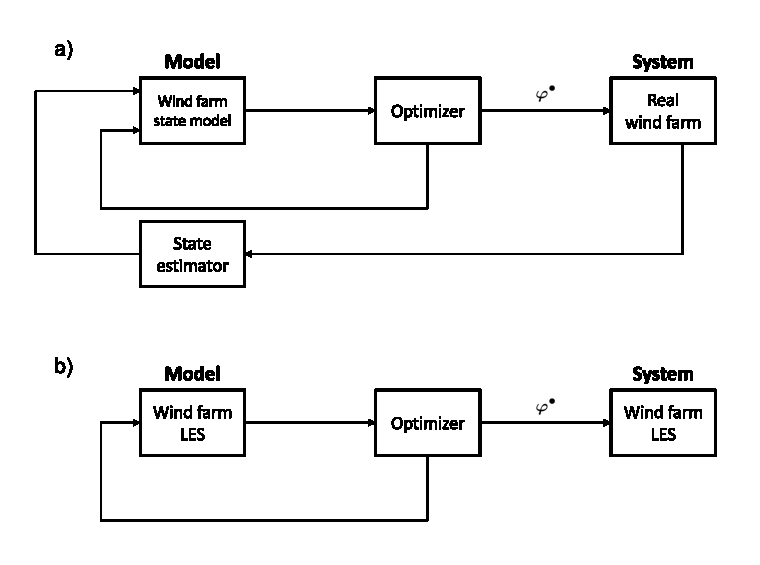
\includegraphics[width=0.6\textwidth]{figure1}
	\caption{Model-predictive control (MPC) applied to wind farms. a) Conventional feedback MPC of a wind farm. b) Benchmark optimal control framework of a wind farm LES considered in the current study. Figure originally published in Munters and Meyers \cite{munters2017optimal} under a CC-BY 4.0 license.}\label{fig:block_diag}
\end{figure}

\begin{figure}
	\centering
	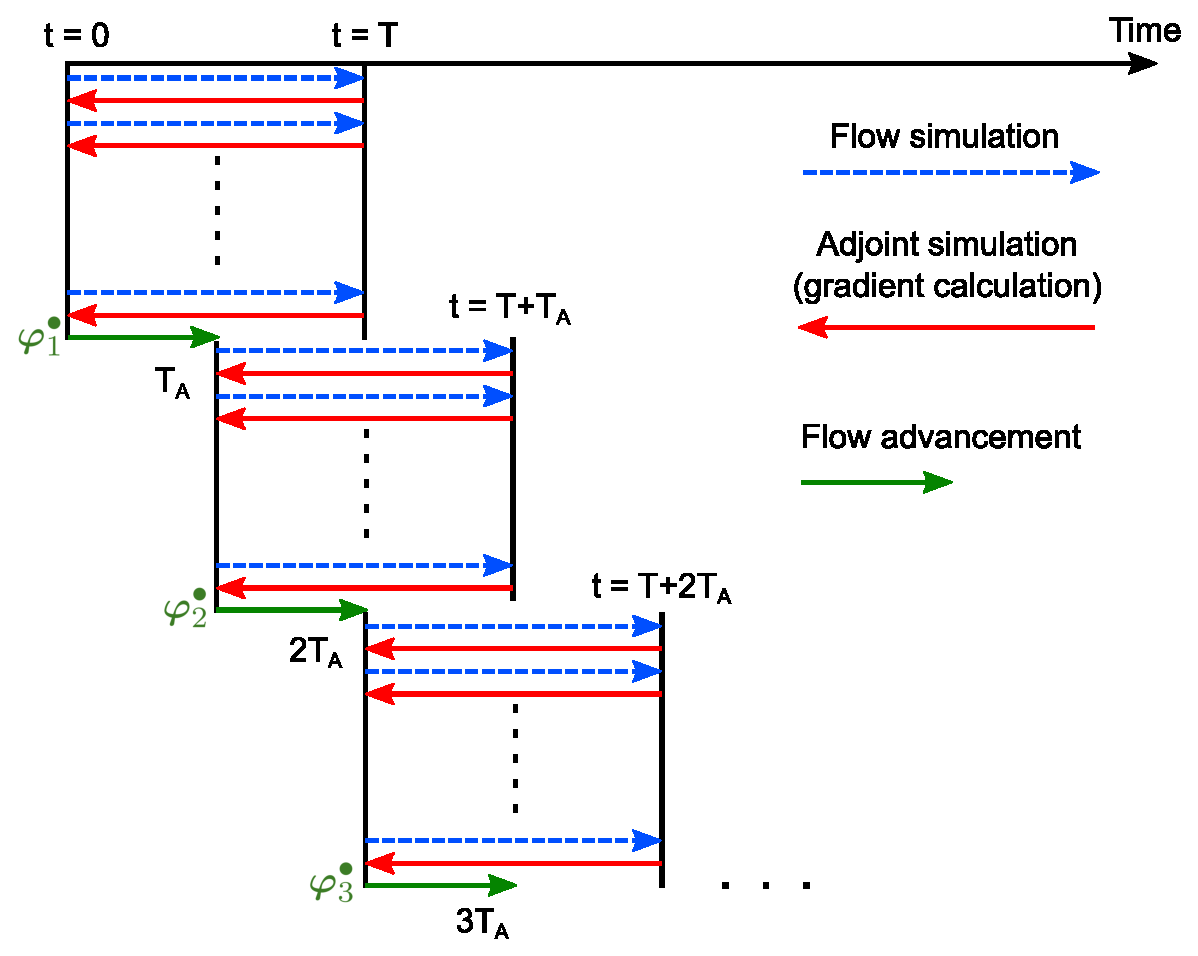
\includegraphics[width=0.55\textwidth]{figure2}
	\caption{Receding horizon framework subdividing time into discrete flow advancement windows of length $T_A$ with prediction horizon $T$. Each arrow represents a forward or adjoint PDE simulation. Each window consists of an optimization stage (blue and red lines), yielding a set of optimal controls $\bs{\varphi}^\bullet$ , followed by a flow advancement stage (green line). Figure originally published in Munters and Meyers \cite{munters2017optimal} under a CC-BY 4.0 license. \label{fig:receding_horizon}}
\end{figure}

In contrast, the current manuscript follows the approach first introduced by Goit and Meyers \cite{goit2015optimal}: instead of focusing on developing a practically realizable wind-farm controller, wind-farm performance is optimized directly in an accurate model with full state information (see, e.g. Refs. \cite{goit2015optimal,goit2016optimal,munters2016effect,munters2017optimal}), i.e. using large-eddy simulations of the filtered Navier--Stokes equations (see Figure \ref{fig:block_diag}b). In this way, instead of being parametrized, the turbulent interactions between wind turbines and the atmospheric boundary layer flow are explicitly resolved using adequate spatio-temporal resolution. In this way, the wind turbines can be used as flow actuators: by dynamically controlling individual thrust setpoints and yaw rates of the turbines we aim to optimally influence the ABL flow such that aggregate wind-farm power extraction is maximized.  Note that this approach is unfeasible for practical control, both due to excessive computational cost and the incomplete state information in practice. However, it allows to benchmark the potential of increasing energy through wind-farm control, and can help identify control mechanisms to be harnessed by practical controllers. Also here, a receding-horizon methodology is used. Within each control window, we consider the following PDE-constrained optimal control problem, in which we maximize the aggregate wind-farm power over a time horizon $T$:

{\small
\begin{alignat}{4}
& \underset{\bs{\varphi}, \bs{q}}{\text{minimize}}  & \qquad  \J(\bs{\varphi}, \bs{q}) &= - \Tint \sum_{i=1}^{N_t} \frac{1}{2} C_{P,i}'~V_i^3 A_i \dt  & \label{eq:costfunction}\\
& \text{s.t.}                      			&         \frac{\partial \utilde}{\partial t} + \big(\utilde \cdot \nabla \big)~ \utilde &= - \nabla (\ptilde + \ptilde_\infty) / \rho - \nabla \cdot \boldsymbol{\tau}_{sgs} + \sum_{i=1}^{N_t} - \frac{1}{2} \ctihat~V_i^2 \R_i(\bs{x})~\eperpi \qquad  & \text{in } \Omega \times (0,T], \label{eq:NSmomentum_constraint} \\
&                                                   &        \nabla \cdot \utilde&=0 									        & \text{in } \Omega \times (0,T], \label{eq:NScontinuity_constraint}\\
&                                                   &        \tau \ddt{\ctihat}&=\cti - \ctihat 								& i=1\dots N_t~\text{in } (0,T],  \label{eq:ctihat_constraint}\\
&                                                   &        \ddt{\theta_i}&=\omega_i											& i=1\dots N_t~\text{in } (0,T],  \label{eq:omega_constraint}\\
&                                                   &        C_{T,\text{min}}' \leq~ &\cti \leq C_{T,\text{max}}'				& i=1\dots N_t~\text{in } (0,T],  \label{eq:boxct_constraint}\\
&                                                   &        -\omega_{\text{max}} \leq~ &\omega_i \leq \omega_{\text{max}}.   	& i=1\dots N_t~\text{in } (0,T].  \label{eq:boxomega_constraint}
\end{alignat}
}

\noindent The ABL state equations in Eq. \eqref{eq:NSmomentum_constraint} - \eqref{eq:NScontinuity_constraint} are the filtered Navier-Stokes equations, which are solved using LES. In these equations, $\utilde$ and $\ptilde$ are the filtered velocity and modified pressure respectively. Furthermore, $\bs{\tau}_{sgs}$ is the subgrid-scale stress tensor, which is modeled using a constant-coefficient Smagorinsky model. The LES solver applies a Fourier spectral discretization in the horizontal directions combined with a energy-conservative fourth order finite-difference scheme in the vertical direction. Inflow conditions are specified using a fringe region method \cite{munters2016turbulent}. Further details regarding the LES solver used in this work can be found for instance in Refs. \cite{meyers2007evaluation, meyers2010large, calaf2010large}.

The wind turbine rotors are modeled using a standard non-rotating actuator disk model (see, e.g., Ref \cite{meyers2010large}). \revision{Turbine towers are not included.} For each turbine $i (= 1 \dots N_t)$, two state variables are defined. First, the turbine thrust coefficient $\ctihat$ is obtained by applying a one-sided exponential time-filter with time constant $\tau$ to the thrust coefficient control setpoint $\cti$ (Equation \ref{eq:ctihat_constraint}). Second, the turbine yaw angle $\theta_i$ is defined in a straightforward way using the yaw rate control $\omega_i$ (Equation \ref{eq:omega_constraint}). Subsequently, the thrust force enacted by the turbine upon the flow can be parametrized as $\bs{f}_{i}(\bs{x}) = - (1/2) \ctihat V_i^2 \R_i (\bs{x}) \eperpi$. Here, $\R_i(\bs{x}) = \sint G(\bs{s} - \bs{x})~H\big[D/2 - \vert\vert \bs{s} - \bs{t}_i \vert\vert_2\big]~\diracdelta \big[ (\bs{s} - \bs{t}_i)\cdot \eperpi \big] \ds$ is a smoothed geometric footprint of the rotor with diameter $D$ at location $\bs{t}_i$ on the LES grid, using a Gaussian kernel $G$ with characteristic filter width $\Delta$. Further, $V_i = (1/A_i) \int_{\Omega} \R_i(\bs{x}) \utilde \cdot \eperpi \dx$ is the axial velocity averaged over the rotor disk with area $A_i$, and the rotor-perpendicular unit vector $\eperpi = \ex \cos \theta_i + \ey \sin \theta_i$ defines the orientation of the rotor disk using the yaw angle state $\theta_i$. Analogously, a rotor-parallel unit vector $\etransi = - \bs{e}_x \sin \theta_i + \bs{e}_y \cos \theta_i$ is defined, which will be used further below. The power extraction of the turbine is calculated as $P_i = (1/2) C_{P,i}' V_i^3 A_i$, with power coefficient $C_{P,i}' = a \ctihat$. The coefficient in the latter linear relation is set to $a = 0.9$ to mitigate overprediction of turbine power on present-day simulation grids as discussed in Ref. \cite{munters2017optimal}. Both the thrust coefficient setpoint controls $\cti$ and the yaw rate controls $\omega_i$ are subjected to technical box constraints in Equations \eqref{eq:boxct_constraint} - \eqref{eq:boxomega_constraint}. As discussed in Section \ref{sec:case_definition} and Table \ref{tab:case_definition}, the control cases considered in this manuscript are differentiated based on the parameter values of these box constraints. The system states are grouped in the vector $\bs{q} = [\utilde(\bs{x},t),~\ptilde(\bs{x},t),~\ctnhat{1}(t), \dots, \ctnhat{N_t}(t),~ \theta_1(t), \dots, \theta_{N_t}(t)] = [\utilde(\bs{x},t),~\ptilde(\bs{x},t),~\widehat{\bs{C}}_T'(t) ,~ \bs{\theta}(t)]$ and the controls, consisting of the individual unsteady thrust coefficient setpoints and yaw rates of every turbine, are denoted as $\bs{\varphi} = [\bs{C}_T'(t),~\bs{\omega}(t)]$.%[\ctn{1},\dots,\ctn{N_t},~\omega_1,\dots,\omega_{N_t}]$. 

As is common practice in PDE-constrained optimization, the problem is solved in a reduced formulation: the dependency of the state variables on the controls, i.e. $\bs{q}(\bs{\varphi})$, is explicitly satisfied by fulfilling the state equations in every step throughout the optimization process, which allows to solve a reduced control-space optimization problem in which the reduced cost functional $\tilde{\J}(\bs{\varphi}) \equiv \J \big(\bs{\varphi},\bs{q}(\bs{\varphi}) \big)$ is minimized, subject only to the box constraints in equations \eqref{eq:boxct_constraint} - \eqref{eq:boxomega_constraint}. The latter problem is solved using the \revision{L-BFGS-B (limited-memory Broyden--Fletcher--Goldfarb--Shanno with bounds support) algorithm \cite{byrd1995limited}}, which is an iterative quasi-Newton algorithm that uses gradient information to construct and optimize a quadratic model of the cost functional in each iteration while attempting to satisfy the strong Wolfe conditions \cite{wolfe1969convergence}. As shown in Figure \ref{fig:receding_horizon}, within each optimization window, the iterative procedure hence results in repeated alternating evaluations of the cost functional (i.e. flow simulations using LES) and gradient (i.e. adjoint simulations, see below).

Instead of using a classical finite-difference gradient approximation to determine $\nabla \tilde{\J}$, which would require a perturbed LES for every dimension in $\bs{\varphi}$ (typically in the order of $10^4$--$10^5$), the gradient is calculated using the continuous adjoint method. The adjoint methodology is widespread in PDE-constrained optimization since it allows to quantify sensitivities of the cost functional to control parameters at a computational expense independent of control space dimensionality (see, e.g., Refs. \cite{jameson1988aerodynamic,giles2000introduction,troltzsch,borzinschulz}). The cost functional sensitivity is calculated by deriving and solving an auxiliary set of equations related to the original state equations, called the adjoint equations:
 
{\small
\begin{align}
- \frac{\partial \bs{\xi}}{\partial t} + \big( \nabla \utilde \big)^T \bs{\xi} - \big( \utilde \cdot \nabla \big) \bs{\xi} &= - \nabla \pi / \rho - \nabla \cdot \boldsymbol{\tau}^*_{sgs} + \sum_{i=1}^{N_t} \bs{f}_i^* & \text{in } \Omega \times (0,T] \label{eq:adjoint_momentum}\\
\nabla \cdot \bs{\xi} &= 0 & \text{in } \Omega \times (0,T]\label{eq:adjoint_continuity}\\
-\tau \ddt{\sigma_i} &= -\sigma_i + \frac{1}{2} V_i^2  (a V_i - X_i) A_i  &  i=1\dots N_t~\text{in } (0,T] \label{eq:adjoint_sigma}\\
- \ddt{\eta_i} &= \frac{1}{2} \ctihat V_i ~ \Bigg[ \int_{\Omega} \bigg((~3 V_i - 2 X_i ) \utilde - V_i \bs{\xi} 
\bigg) \cdot \bs{e}_{\parallel,i} \R_i \dx ~ \nonumber \\
& \qquad + \sint \bigg( (3 V_i - 2 X_i )~\utilde - V_i \bs{\xi} \bigg) \cdot \eperpi ~ \mathscr{Q}_i  \dx \Bigg] &  i=1\dots N_t~\text{in } (0,T] \label{eq:adjoint_eta}.
\end{align}
}

\noindent In these equations $\bs{\xi}$, $\pi$, $\sigma_i$, and $\eta_i$ are the adjoint variables associated with the state variables $\utilde$, $\ptilde$, $\ctihat$, and $\theta_i$ from the original optimal control problem. Further, $X_i$ is the adjoint disk-averaged velocity defined analogously to its forward version $V_i$, and $\bs{f}_i^* = \frac{1}{2} \ctihat V_i (~3a V_i - 2 X_i ) \R_i \eperpi$ is the adjoint turbine forcing. The rotational rotor footprint $\mathscr{Q}_i$ from Equation \eqref{eq:adjoint_eta} is defined as 

\begin{equation}
\mathscr{Q}_i = \sint \frac{12 (\bs{s} - \bs{x})\cdot \eperpi}{\Delta^2} G(\bs{s} - \bs{x})  H\big[D/2 - \vert\vert \bs{s} - \bs{t}_i \vert\vert_2 \big] \diracdelta\big[(\bs{s} - \bs{t})\cdot \eperpi \big]  (\bs{s} - \bs{t}_i) \cdot \etransi \ds,
\end{equation} 

%\noindent and quantifies the dependence of the rotor footprint $\R_i$ on the yaw angle $\theta_i$. A further interpretation and illustration of this term is given in the Appendix. The derivation of the standard transport terms in the adjoint Navier-Stokes equations is well established in literature (see, e.g. Refs. \cite{bewley2001dns, choi1999instantaneous}). For the derivation of case-specific terms, such as the adjoint subgrid-scale Smagorinsky model, adjoint turbine forcing, and adjoint thrust coefficient (Equation \ref{eq:adjoint_sigma}), we refer the reader to Refs. \cite{goit2015optimal} and \cite{munters2017optimal}. The adjoint fringe forcing technique, facilitating non-cyclic adjoint simulations, is elaborated in Goit \emph{et al.} \cite{goit2016optimal}. Finally, the adjoint yaw angle equation for $\eta_i$ (Equation \eqref{eq:adjoint_eta}) is newly presented in this work, and is derived in the Appendix. Upon satisfaction of the adjoint equations, the adjoint variables $\bs{q}^* = [\bs{\xi}(\bs{x},t),~\pi(\bs{x},t),~\bs{\sigma}(t),~\bs{\eta}(t)]$ are subsequently used to form straightforward analytical expressions for the gradient as 



\begin{equation}
\nabla \Jtilde \equiv 
\begin{bmatrix*}[l]
\partial \Jtilde / \partial \bs{C}_T' \\
\partial \Jtilde / \partial \bs{\omega} 
\end{bmatrix*} = 
\begin{bmatrix}
- \bs{\sigma}\\
- \bs{\eta}
\end{bmatrix} \label{eq:problem_gradient}.
\end{equation}



\section{Numerical setup and case description}\label{sec:opt_yaw_setup}
\noindent This section discusses the simulation cases and setup details that will be used to assess the potential of dynamic yaw control. A wind farm of 16 wind turbines with a rotor diameter $D = 100$ m is considered. The turbines are arranged in a $4 \times 4$ aligned pattern, with $6D$ spacing in both axial and transversal directions. First, numerical setup parameters for the simulation and optimization are discussed. Next, the different control cases are introduced. 

\subsection{Simulation setup}\label{sec:num_setup}
\noindent The simulation domain has a \revision{total dimension of $L_x \times L_y \times L_z = 4.8 \times 2.4 \times 1 $ km$^3$, with $L_x, L_y$, and $L_z$ the streamwise, transversal, and vertical extent of the domain respectively. This domain is discretized on a grid of $N_x \times N_y \times N_z = 256 \times 128 \times 128$ gridpoints.} The final $10\%$ of the streamwise extent of the domain is used as a fringe region to impose inflow conditions. All cases apply periodic boundary conditions on transversal domain boundaries. 

Two different sets of simulations are considered. The first set is subjected to a \revision{constant} and uniform inflow with $U_\infty = 8$ m s$^{-1}$. In this case, the top and bottom boundaries are treated with a symmetry condition, \revision{and the vertical location of the turbine hubs $z_h$ is placed at the vertical mid-plane of the domain, i.e. $z_h/L_z = 0.5$,} in order to minimize any influence of vertical domain boundaries. The second set applies unsteady turbulent inflow conditions, which are generated in a pressure-driven precursor simulation of an unperturbed turbulent boundary layer with shifted periodic boundary conditions \cite{munters2016shifted}, driven by a pressure gradient forcing of $\partial_x p_\infty/\rho = 2.5 \times 10^{-4}$ m s$^{-2}$. This results in a freestream wind speed at hub height fluctuating slightly above 8 m s$^{-1}$. In this second set of simulations, the top boundary is treated with a stress-free condition, and a high-Reynolds number wall model is used at the bottom. The turbines are placed at a height of $z_h/L_z = 0.1$ from the wall. The wall model adds a wall stress consistent with a rough-wall logarithmic boundary layer profile with roughness length $z_0/L_z = 10^{-4}$, resulting in a inflow turbulence intensity of about 8\% at hub height. 

\revision{Within the context of the receding-horizon methodology introduced in Section~\ref{sec:meth}, the optimization is performed over discrete time windows with optimization horizon $T$ and flow advancement time $T_A$. Ideally, one would take a very large optimization horizon $T$, and a small flow advancement time $T_A$ before recomputing the optimal control problem. However, in practice, $T$ is limited due to the inherent chaotic nature of turbulent flows that complicates control over long time horizons, and $T_A$ should not be taken too small to avoid excessive computational costs. In the current work, we use 6 consecutive windows, each with an optimization horizon $T=300$~s and a flow advancement time of $T_A = T/2= 150$~s, resulting in a total control time of 900~s. Note that, given a wind-farm length of $3 \times 6D = 1 800$ m and a free-stream velocity $U_\infty = 8$ m s$^{-1}$, the wind-farm flowthrough time is approximately 225 s. Hence, the total control time comprises about 4 flowthroughs, and the optimization horizon within each window covers about 1.33 flowthrough times. Because of the latter, each turbine row has the opportunity to take into account interaction with every downstream row, and the sensitivity of power gains to the optimization horizon $T$ is expected to be limited.} All time-averaged results shown below are based on statistics gathered after 300~s, so that wake propagation time lag at startup is excluded. To limit computational efforts, we perform a fixed amount of 80 L--BFGS--B iterations in each window, corresponding to approximately 160 PDE simulations (forward or adjoint). Although formal convergence is not achieved for any of the cases after this amount of iterations, it will be shown later that the relative ordering of the cases based on power extraction is clear. Computational costs amount to approximately 35~000 corehours per optimization case for all 6 time windows combined on 112 Intel Broadwell architecture cores connected by an EDR Infiniband network. The initial guess for the optimal controls within each window is a steady thrust coefficient setpoint $C_T'=2$  and yaw rate $\omega = 0^\circ$ s$^{-1}$ for all turbines. \revision{The sensitivity of attainable power gains to $T/T_A$, initial control guesses, and optimizer settings has been shown to be limited in a prior study \cite{munters2017optimal}.} Simulation and optimization parameters are summarized below in Table~\ref{tab:case_definition}.

Simulations are initialized as follows: for the turbulent inflow case, a fully-developed high-Reynolds number turbulent boundary layer is generated in the precursor inflow simulation by simulating a perturbed logarithmic flow until a statistically-stationary state is achieved. For both the turbulent and the uniform inflow cases the main wind-farm simulation is then advanced in time with the proper inflow conditions for approximately five wind-farm flow-through times, after which the effects of wind-farm start-up transients have subsided. These statistically stationary wind-farm flows then serve as initial conditions for the control cases defined below. Planviews at hub height of these initial conditions are shown in Figure~\ref{fig:initial_conditions_flow_yaw}. It can be seen from the Figure~\ref{fig:initial_conditions_flow_yaw}a that, given laminar inflow conditions, turbine wakes are very deep and remain stable up until row 3, after which meandering and vortex shedding starts to occur. These flow conditions can be regarded as somewhat artificial since, in the atmospheric boundary layer, background turbulence typically causes instant wake transition behind the turbine rotor. \revision{Furthermore, it is documented in literature that numerical details such as grid resolution, subgrid-scale modeling, and turbine models can have a significant impact on simulation results , whereas in turbulent inflow this is much less the case  \cite{martinezwake,sarlakwe,troldborgtorque}. In practice, this tends to lead to artificially stabilized wakes with very low farm efficiencies (see, e.g., Refs \cite{sarlaktorque, ciriacc}).} Nevertheless, this setup allows us to investigate control dynamics more easily, as we can rule out any reaction of the optimization to the background variability. Furthermore, suppressed wake meandering and reduced turbulence levels have been known to occur in wind farms submerged in stably stratified atmospheric boundary layers \cite{larsen2009dependence, machefaux2016experimental}, hence rendering the current case somewhat relevant for such situations. Figure~\ref{fig:initial_conditions_flow_yaw}b shows that, for the turbulent inflow case, the background turbulence causes wake instabilities instantly, leading to enhanced wake recovery and much more complex unsteady wake interactions between turbines.

\begin{figure}
	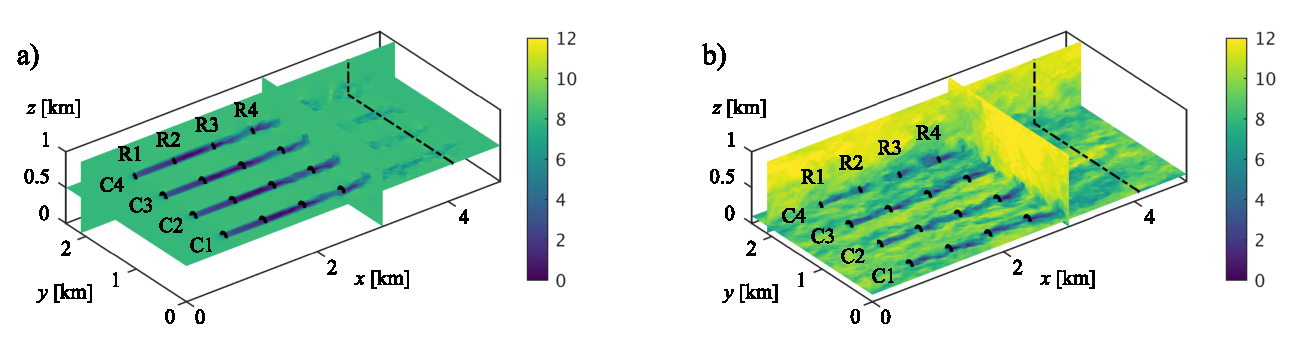
\includegraphics[width=\textwidth]{figure3_revised}
	\caption{Snapshots of initial conditions for optimal control cases. \emph{a)} Uniform and \revision{constant} inflow. \emph{b)} Turbulent inflow. Colors represent instantaneous streamwise velocity $\widetilde{u}_x$ in m s$^{-1}$. The black lines represent wind turbine locations. The black dashed line indicates the start of the fringe region. R1 -- R4 and C1 -- C4 indicate the numbering convention used for turbine rows and columns respectively. \label{fig:initial_conditions_flow_yaw}}
\end{figure}

\subsection{Control cases}\label{sec:case_definition}

\noindent For each set of simulations, a steady reference case (R) with $C_T' = 2$ and $\omega = 0^\circ$/s is considered. In this way, turbines in the reference case remain aligned with the mean-flow direction and operate at Betz-optimal thrust coefficients. Further, a first yaw control case (Y) is defined, with a steady $C_T'=2$, but turbines are allowed to yaw dynamically at a maximum rate of $\omega^{\text{max}} = 0.3^\circ$/s, corresponding to the maximum yaw rate of the conceptual NREL 5MW and the DOWEC 6MW turbines \cite{jonkman2009definition, kooijman2003dowec}. In addition, a second yaw control case (Y5) is constructed, for which a higher maximum yaw rate of $\omega^{\text{max}} = 5^\circ$/s is selected. Although this significantly exceeds the capabilities of the abovementioned turbine design concepts, this case will allow to assess whether significant gains in power could be achieved by rapidly yawing turbine designs, such as low-inertia two-bladed teeter hinge wind turbines \cite{kim2014yaw}. 

Similar to earlier studies \cite{munters2017optimal, munters2016effect}, also two induction control cases are considered, in which turbines can adapt their thrust coefficient $C_T'$ with a characteristic timescale $\tau = 5$ s: an underinductive case where turbines are restricted to lowering $C_T'$ below the Betz-optimal value if desired (I2, with $\ctmax = 2$), and an overinductive case in which also higher $C_T'$ values resulting in increased thrust forces are allowed (I3, with $\ctmax = 3$). Finally, for both the latter cases, also the option of combining dynamic induction control with the yaw control of case Y is considered, defining the yaw--induction cases I2Y and I3Y respectively. The cases investigated in this study are summarized in Table~\ref{tab:case_definition}. 

\begin{table}
	\caption{Setup parameters for optimal dynamic induction and yaw control cases \label{tab:case_definition}}
	\centering
	\begin{tabular}{llccc}
		\toprule
		\multicolumn{5}{l}{\textbf{Simulation parameters}}\\
		\midrule
		Domain size  			& \multicolumn{4}{l}{$L_x \times L_y \times L_z = 4.8 \times 2.4 \times 1$ km$^3$}  \\ 
		Turbine dimensions  		& \multicolumn{4}{l}{$D = 0.1L_z = 100$ m}\\ 
		Turbine spacing  		& \multicolumn{4}{l}{$S_x = 6D, \quad S_y = 6D$}\\
		Windfarm layout 		& \multicolumn{4}{l}{$N_t = 16 $ turbines = 4 rows $\times$ 4 columns} \\ 
		Grid size 			& \multicolumn{4}{l}{$N_x \times N_y \times N_z = 256 \times 128 \times 128$}\\
		Cell size 			& \multicolumn{4}{l}{$\Delta_x \times \Delta_y \times \Delta_z = 18.75 \times 18.75 \times 7.8$ m$^3$}\\
		Time step 			& \multicolumn{4}{l}{$\Delta t = 0.75$ s}\\		
		& & & & \\	
		\multicolumn{5}{l}{\textit{Uniform inflow}}\\
		Hub height & \multicolumn{4}{l}{$z_h/L_z$ = 0.5}\\
		Inflow velocity & \multicolumn{4}{l}{$U_\infty$ = 8 m s$^{-1}$}\\
		& & & & \\			
		\multicolumn{5}{l}{\textit{Turbulent inflow}}\\
		Hub height & \multicolumn{4}{l}{$z_h/L_z$ = 0.1}\\		
		Precursor pressure gradient  	& \multicolumn{4}{l}{$ \partial_x p_\infty \revision{/\rho} = 2.5 \times 10^{-4}$ m s$^{-2}$}  \\ 
		Surface roughness  &  \multicolumn{4}{l}{$z_0 = 10^{-4}H = 0.1$ m}\\ 		
		& & & & \\	
		\toprule
		\multicolumn{5}{l}{\textbf{Optimization parameters}}\\
		\midrule
		Optimization method		& \multicolumn{4}{l}{L--BFGS--B} \\
		Hessian correction pairs	& \multicolumn{4}{l}{$m = 5$} \\
		BFGS iterations 		& \multicolumn{4}{l}{$N_{it} = 80$ ($\approx 160$ PDE)} \\
		Optimization time window	& \multicolumn{4}{l}{$T = 300$ s}\\
		Flow advancement time window 	& \multicolumn{4}{l}{$T_A = 150$ s}\\
		Total operation time         	& \multicolumn{4}{l}{$T_{tot} = 900$ s (6 windows)}\\
		& & & & \\	
		\toprule
		\textbf{Cases} & \  & $C_{T,\text{min}}'$ & $C_{T,\text{max}}'$ & $\omega_{\text{max}}$ [$^\circ/s$] \\ 
		\toprule
		Reference & (R)    &  2 & 2 & 0   \\ 
		Yaw control & (Y)   &  2 & 2 & \textbf{0.3} \\ 
		Fast yaw control & (Y5)   &  2 & 2 &\textbf{5}   \\ 
		Underinduction control & (I2)    &  \textbf{0} & 2 & 0\\
		Overinduction control & (I3)    &  \textbf{0} & \textbf{3} & 0\\ 
		Underinduction + yaw control & (I2Y)   &  \textbf{0} & 2 & \textbf{0.3} \\ 
		Overinduction + yaw control & (I3Y)   &  \textbf{0} & \textbf{3} & \textbf{0.3} \\ 
		\bottomrule
	\end{tabular} 
\end{table}

\section{Results \& discussion}\label{sec:opt_yaw_results}
\noindent The current section presents and discusses the results of the optimal control cases. Firstly, the convergence behavior is illustrated for a typical optimization window in Section~\ref{sec:opt_convergence}, justifying the optimization parameters discussed in previous section. Thereafter, Section~\ref{sec:opt_yaw_uniform} and~\ref{sec:opt_yaw_turb} present the results of the uniform and turbulent inflow cases respectively. Concluding, Section~\ref{sec:opt_yaw_disc} compares both simulation sets and identifies the most promising control approaches.

\subsection{Convergence behavior}\label{sec:opt_convergence}
\noindent Figure~\ref{fig:convergence} illustrates the convergence behavior within the second optimization window of the \revision{turbulent} inflow case. Figure~\ref{fig:convergence}a shows that, although formal convergence is not achieved for any of the cases, after 80 iterations, the relative ordering of the cases is clear and we assume that further improvements in the cost function for an increased amount of iterations are marginal. From Figure~\ref{fig:convergence}b it can be seen that the amount of PDE evaluations (forward or adjoint) is approximately twice the amount of BFGS iterations, indicating that the optimizer mostly takes Newton steps without a further line search. Similar characteristics were observed for the \revision{uniform} case (not further shown here).

\begin{figure}
	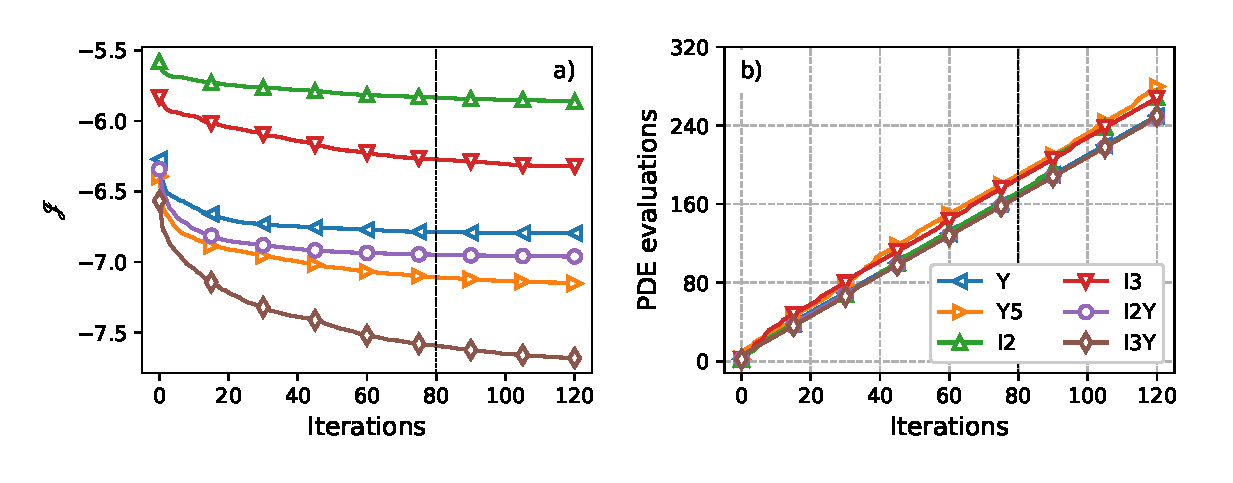
\includegraphics[width=\textwidth]{figure4_revised}
	\caption{Convergence behavior for the second optimization window in \revision{turbulent} inflow. \emph{a) }: Cost functional $\mathscr{J}$. \emph{b) }: PDE evaluations (forward or adjoint). Markers represent every fifteenth iteration step.\label{fig:convergence}}
\end{figure}

\subsection{Uniform inflow}\label{sec:opt_yaw_uniform}
\noindent Figure~\ref{fig:flowfield_uniform} depicts instantaneous planviews of velocity and vorticity at hub height at \revision{t = 300~s} for the reference case R, yawing case Y, overinductive case I3, and combined case I3Y. 
A first qualitative comparison between flow fields illustrates different mechanisms for increasing power extraction. Yawing case Y achieves wake direction, mixing, and later spreading through reorientation of turbine thrust forces. In contrast, overinductive case I3 increases mixing by periodically shedding vortex rings from upstream turbines, as indicated by the regions of increased vorticity in the turbine wakes. Similar behavior was identified from the analysis of prior induction control studies \cite{muntersphd}. Combined yaw--induction case I3Y shows a superposition of the aforementioned behavior, i.e. redirected wakes with periodically shed vortices. 


\begin{figure}
	\includegraphics[width=\textwidth]{figure5_revised}
	\caption{Instantaneous planviews at hub height for uniform inflow cases R, Y, I3, and I3Y at \revision{$t= 300$~s}. \emph{Top: } Streamwise velocity. Coloring in m s$^{-1}$. \emph{Bottom: } Wall-normal vorticity. Coloring in s$^{-1}$. \label{fig:flowfield_uniform}}
\end{figure}

First, in \S\ref{subsec:uni_powerextr} time-averaged power extraction and wind-farm efficiency are compared between cases. Second, in \S\ref{subsec:uni_yaw} yaw characteristics of the yaw-enabled control cases Y, Y5, I2Y, and I3Y are discussed. Time evolution of yaw angles is shown, and two distinct yawing regimes are identified. Finally, the induction characteristics of induction-enabled cases I2, I3, I2Y, and I3Y are shortly presented in \S\ref{subsec:uni_induction}.

\subsubsection{Power extraction and wind-farm efficiency}\label{subsec:uni_powerextr}
\noindent Figure~\ref{fig:power_uniform} illustrates time-averaged wind-farm power results. Figure~\ref{fig:power_uniform}a shows the row-averaged power extraction of the optimal control and reference cases, normalized by first-row power in the reference case $\overline{P}_{R1}^R$. It is shown that all cases curtail first-row power by about $10-20\%$ to the benefit of downstream rows. Furthermore, yaw-enabled cases Y, Y5, and IY achieve an almost flat power curve among rows, and significantly outperform the exclusively inductive cases I2 and I3, for which modest gains are obtained only in the second and third row. Note especially the last row of case I3Y, which achieves a power extraction close to freestream conditions. \revision{Remark that the favorability of yaw over induction control is quantified here for a relatively small set of aligned, and care should be taken when extrapolating these results to wind farms of larger size and/or different layouts (see further discussion in Section \ref{sec:opt_yaw_concl}).}

Figure~\ref{fig:power_uniform}b depicts the wind farm efficiency, defined with respect to a situation in which all turbines extract the same power as a first-row reference case turbine, i.e. $\eta_{\text{farm}} = \overline{P}_{\text{farm}}/(N_t \overline{P}_{R1}^{R})$. As expected \revision{from the discussion in Section \ref{sec:num_setup}}, the efficiency of the uncontrolled reference farm R is very low at around $40\%$.  The inductive cases I2 and I3 manage to increase the efficiency to approximately 50\%, whereas the standard yawing case Y attains an overall efficiency of about 77$\%$. Further, it can be seen that, under uniform inflow conditions, adding the possibility of fast yawing (case Y5) or underinduction (case I2Y) yields only a very minor increase in wind-farm efficiency compared to case Y. In contrast, the combined overinductive yaw control from case I3Y results in a significantly higher efficiency of about 84\%, indicating the potential for combining these control strategies under uniform inflow. The figure also includes results for two additional control cases that are based on simplified controls derived from the yaw characteristics of the optimal control case Y. \revision{Firstly, Ystat denotes a static yaw control case based upon the time-averaged yaw angles of case Y. Secondly, Ymndr is a dynamic yaw control case in which the first-row turbines performs small yaw rotations in an alternating directions.} These simplified control cases are further detailed and discussed below.

\begin{figure}
	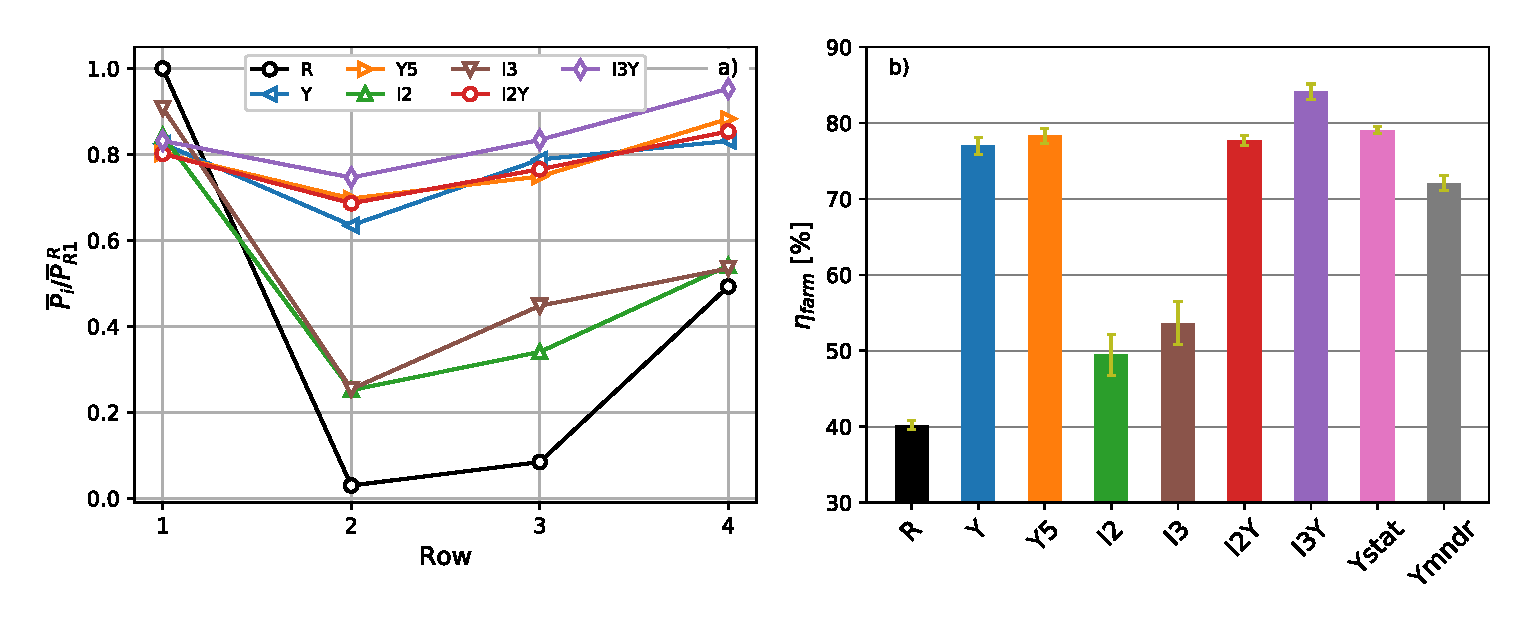
\includegraphics[width=\textwidth]{figure6}
	\caption{\revision{Wind-farm power extraction for reference case R, optimal control cases (Y, Y5, I2, I3, I2Y, and I3Y), and derived control cases (Ystat and Ymndr, see further description below)}. \emph{a) } Row-averaged power, normalized by first-row power of reference case R. \emph{b) } Wind-farm efficiency $\eta_{\text{farm}}$ compared to situation in which all turbines are first-row turbines of R case. Errorbars indicate confidence intervals of $\pm$ 2 standard deviations and are calculated using the procedure detailed in Appendix~C of Ref. \cite{munters2017optimal}. \label{fig:power_uniform}}
\end{figure}

\subsubsection{Yaw characteristics}\label{subsec:uni_yaw}
\noindent Figure~\ref{fig:dynamic_uniform} illustrates the time evolution of normalized power extraction and yaw angle \revision{for columns C2 and C4} of the optimal yawing cases (Y, Y5, I2Y, and I3Y), as defined in Table~\ref{tab:case_definition}. \revision{Columns C1 and C3 show similar behavior to either C2 or C4, and are omitted from the Figure for clarity of presentation. } The top panels of Figure~\ref{fig:dynamic_uniform} show that, for all optimal yaw cases, power is curtailed to a limited extent in the first row, whereas power in downstream rows is increased significantly after a delay corresponding to the wake advection time.  
\begin{figure}
	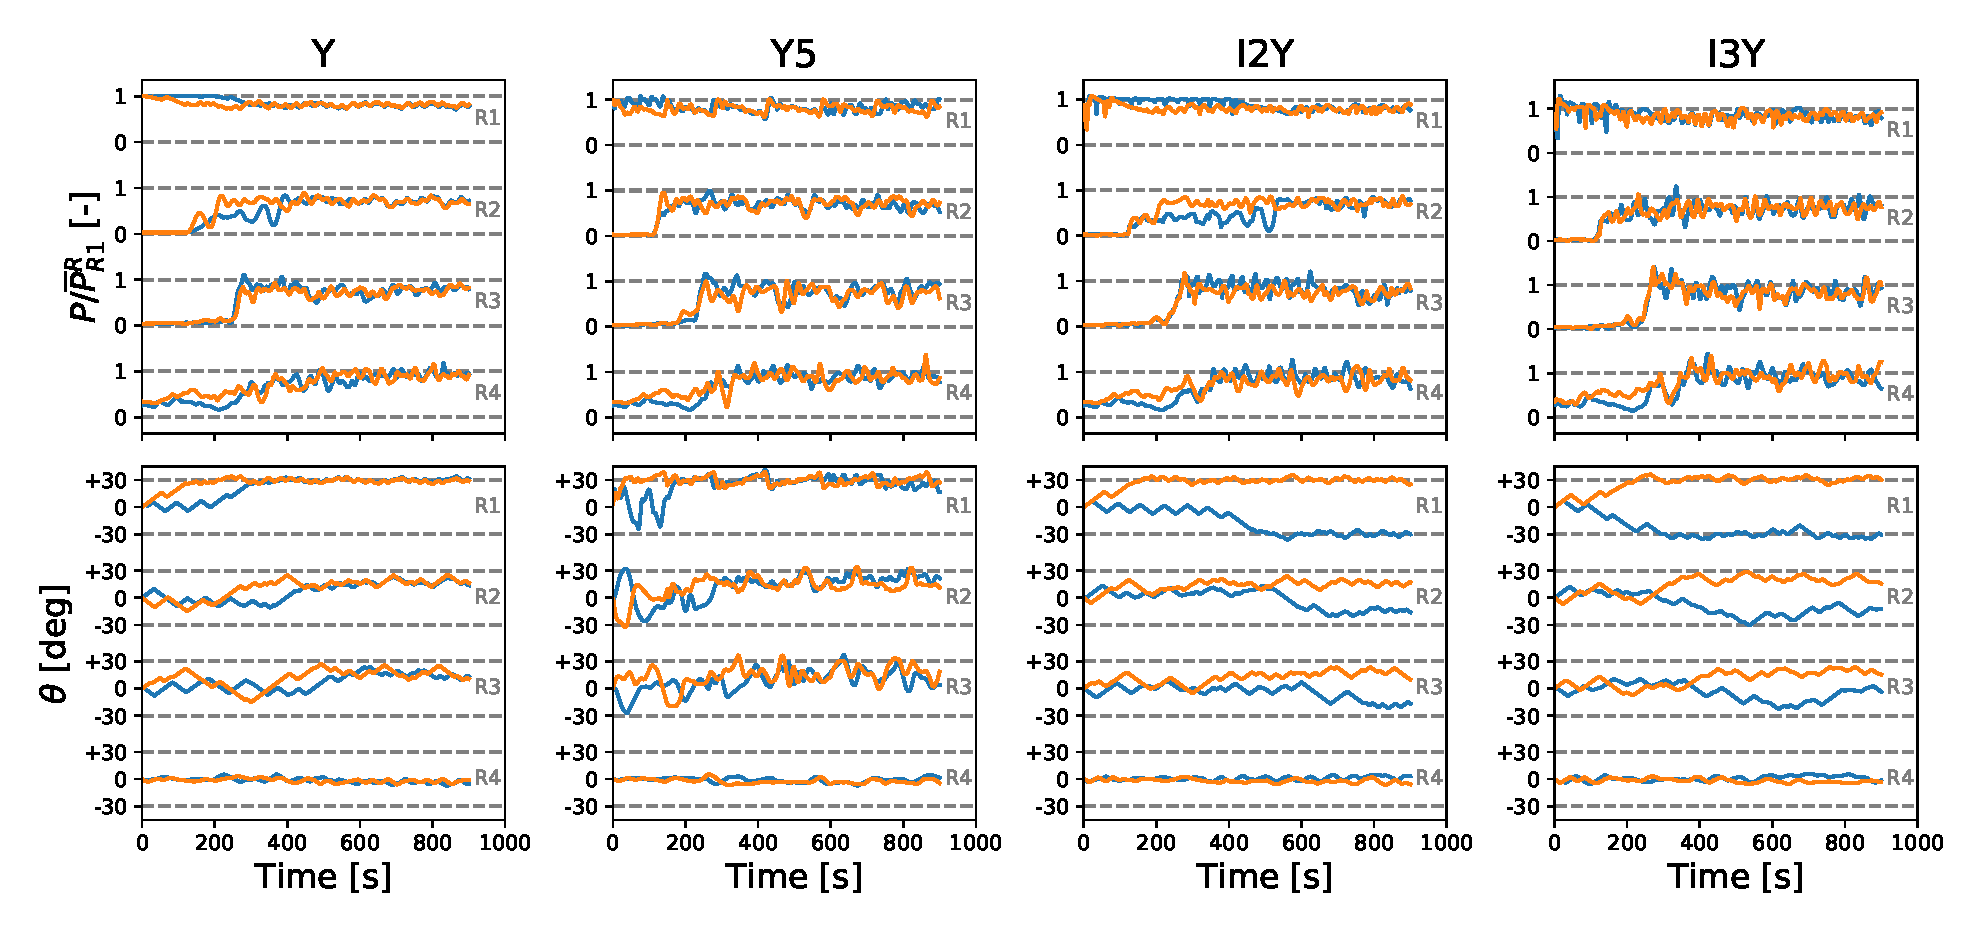
\includegraphics[width=\textwidth]{figure7_revised}	
	\caption{Time evolution of uniform inflow yaw-enabled cases for turbine columns C1 and C4. \emph{Top: } Turbine power extraction $P$, normalized by mean first row power in the uncontrolled reference $\overline{P}_{R1}^R$. \emph{Bottom: } Yaw angle $\theta$. Line colors indicate different turbine columns {\color{C1} C2} and {\color{C2} C4} as indicated in Figure~\ref{fig:initial_conditions_flow_yaw}, i.e. every line represents a single wind turbine. \label{fig:dynamic_uniform}}
\end{figure}

Turning to the time evolution of the yaw angle $\theta$, a first observation is that, although the four columns of the considered wind farm are \emph{statistically} equivalent in the reference case, their behavior in an optimal control setting is heterogeneous. \revision{The reason for this is that the cost functional gradient used in the optimization process is based on the instantaneous flow conditions through the adjoint equations. These conditions are not the same for different columns, e.g. the turbulence in the wakes behind the third row observed in Figure \ref{fig:flowfield_uniform} is different for every column, which can cause the optimizer to converge to a different dominant control mechanism in different columns.} For example, for cases Y \revision{and I2Y}, the first-row behavior of the yaw angle $\theta$ seems to exhibit a bifurcation between two limit cycles. On the one hand, the first-row turbines in column C2 initially oscillates around the flow-aligned yaw angle of $0^\circ$, triggering a \emph{wake meandering} type of motion. \revision{Similar behavior was observed for columns C1 and C3.} Column C4 on the other hand directly turns to a misaligned yaw angle of $30^\circ$, after which it shows some minor high frequency yaw oscillations. As shown in panel Y of Figure~\ref{fig:flowfield_uniform}, the former wake meandering mechanism mainly acts on increased wake spreading in the lateral direction \revision{(columns C1, C2, and C3)}, and enhances recovery by increasing the contact area between the wake and its surroundings. Turbine row 2 and 3 show more complex oscillations, with additional variability in response to the unsteadiness in local flow conditions. In contrast, the first-row yaw misalignment in column C4 creates a more shallow wake which is \emph{redirected} such that it just misses the downstream turbine. Downstream rows 2 and 3 exhibit some minor oscillations around a yaw misalignment angle of $\approx 17^\circ$, causing further yaw redirection downstream. Since there is no further downstream potential for wake mixing or redirection, the final row consistently shows a yaw angle aligned with the mean flow. Similar time evolutions of the yaw angle are observed for column C2 of the combined yaw--induction case I2Y. \revision{In cases I3Y and Y5, the wake redirection regime is dominant, except for the very early stage of the time window}. In summary, two distinct and relatively simple mechanisms for power increase through yaw control are found: on the one hand a \emph{dynamic} wake meandering regime is identified, and on the other hand a \emph{static} wake redirection regime is observed. These mechanisms are further analyzed below.

\paragraph{Static yaw regime - wake redirection}
\noindent Figure~\ref{fig:cross_section} shows cross sections of the time-averaged axial velocity field from case~Y, taken at half a rotor diameter upstream of rows 2, 3, and 4 in column C4, for which turbines directly go to static yaw angles of 30$^\circ$, 17$^\circ$, and 17$^\circ$ for the first, second, and third row respectively (see Figure~\ref{fig:dynamic_uniform}). The figure illustrates that the yaw misalignment of upstream turbines causes the wake to be redirected away from the downstream ones. Moreover, as observed in recent studies, the wake induced by the yaw-misaligned upstream turbines has a curled shape with counter-rotating vortices at its top and bottom \cite{howland2016wake,bastankhah2016experimental}. The current LES-based flow model allows to directly account for this in developing the control strategies, as the wakes are curled just around the downstream turbines, resulting from a trade-off between limiting upstream power loss and redirecting the wakes sufficiently. \revision{It is important to note that such wake redirection and curling is not simply an artifact of the currently used non-rotating ADM, since similar wake characteristics were also observed in rotating actuator line models \cite{howland2016wake}.} The static yaw wake redirection regime observed in the optimal control simulations can be mimicked by imposing fixed yaw misalignments corresponding to the aforementioned values. This simplified control case is denoted as Ystat. 

It can be seen from Figure~\ref{fig:power_uniform}b that Ystat yields approximately the same wind-farm efficiency of 79\% as the optimally controlled yawing cases Y and Y5, suggesting that, for the uniform inflow case, any dynamic effects observed for turbines in the wake redirection regime are of very minor importance. Furthermore, the fact that the expected value of Ystat is slightly higher than that of Y and Y5 can be attributed to the fact that optimizations are not fully converged, finite-horizon effects possibly have a small negative influence on the optimal control cases, and the wake meandering regime that is present in some turbines for the optimal control cases yields slightly lower power than the pure wake redirection of Ystat.

\begin{figure}
	\includegraphics[width=\textwidth]{figure8}
	\caption{Time-averaged cross-sectional views of streamwise velocity $\widetilde{u}_x$ for case Y at a distance $D/2$ upstream of the downstream turbines in column C4. Arrows represent the projection of the velocity vector on the cross-sectional plane. Dashed white lines indicate turbine rotor locations. Coloring in m s$^{-1}$. \label{fig:cross_section}}
\end{figure}

\paragraph{Dynamic yaw regime - wake meandering}
\noindent Figure~\ref{fig:spec_uniform} shows row-averaged yaw angle power spectral densities $S_{\theta \theta}$. We focus on relatively slow dynamics: spectra are shown up to a Strouhal number $St = f D/U_\infty = 0.8$, corresponding to variations with a time period longer than 15 s. The figure shows that, for the upstream rows 1 to 3, the variance of the fast yawing case Y5 is significantly higher than the slow yawing cases Y, I2Y, and I3Y. The first row of case Y shows a significant peak around $St = f D/U_\infty= 0.2$, corresponding to the frequency of the aforementioned oscillations around aligned yaw angles, triggering wake meandering. Smaller subsequent peaks at harmonics of this frequency are also observed. Indeed, a Strouhal number in the range of 0.1 -- 0.3 has been associated with natural wake meandering before in various studies \cite{medici2008measurements, howard2015statistics}. Although attenuated, this peak seems to manifest itself to a limited degree in downstream rows as well. Furthermore, traces of this behavior are also observed for case I2Y, for which it was already mentioned that the first row of column C2 showed behavior consistent with a regime triggering wake meandering. In contrast, as observed qualitatively from Figure~\ref{fig:dynamic_uniform}, cases Y5 and I3Y show no strongly coherent dynamic yaw characteristics, indicating that static wake redirection yaw is dominant here. Similar to the simplified static yaw case derived from the wake redirection behavior in previous paragraph, the wake meandering regime can be approximated by imposing a simple bang-bang control on the first row turbines, with an alternating yaw rate $\omega = 0.3^\circ$ s$^{-1}$ in both directions with a frequency corresponding to a Strouhal number $St = 0.2$. The coherent dynamics and phase differences of the yaw rates in the downstream turbines are more complex. Therefore, these turbines are not yawed in the derived control case. This simplified case is further denoted as Ymndr. Figure~\ref{fig:power_uniform}b illustrated that, by simply applying this bang-bang control in the first-row turbine, a wind-farm efficiency of about 72\% can be attained.

\begin{figure}
	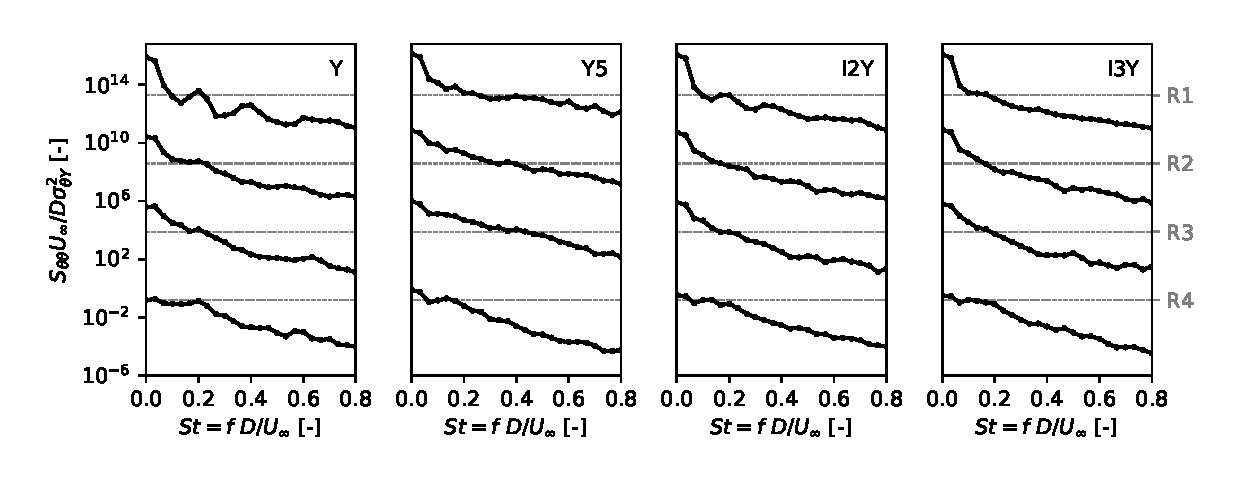
\includegraphics[width=\textwidth]{figure9_revised}
	\caption{\revision{Row-averaged yaw angle power spectral densities $S_{\theta \theta}$ as a function of Strouhal number $St = f D/U_\infty$. Spectra of different rows are shifted vertically for clarity. Horizontal dashed lines indicate identical reference values for each row. Spectra are non-dimensionalized using $\sigma_{\theta Y}^2$, the row-averaged variance of the first row yaw angles in case Y.}\label{fig:spec_uniform}}
\end{figure}


\subsubsection{Induction characteristics}\label{subsec:uni_induction}
\noindent Figure~\ref{fig:dynamic_ctfilt} illustrates the time evolution of normalized power extraction and thrust coefficient of the optimal induction cases (I2, I3, I2Y, and I3Y), as defined in Table~\ref{tab:case_definition}. In contrast to the heterogeneous behavior in different columns for the yaw angles as shown in Figure~\ref{fig:dynamic_uniform} above, the induction coefficient behavior is similar for each column, and is illustrated for column C1 only. The top panels of Figure~\ref{fig:dynamic_ctfilt} indicates that, for the exclusively inductive cases I2 and I3, first-row power is pulsed severely, leading to intermittent increases in downstream power extraction. This differs from the combined yaw--induction cases, which show much smoother power extraction dynamics. 
\begin{figure}
	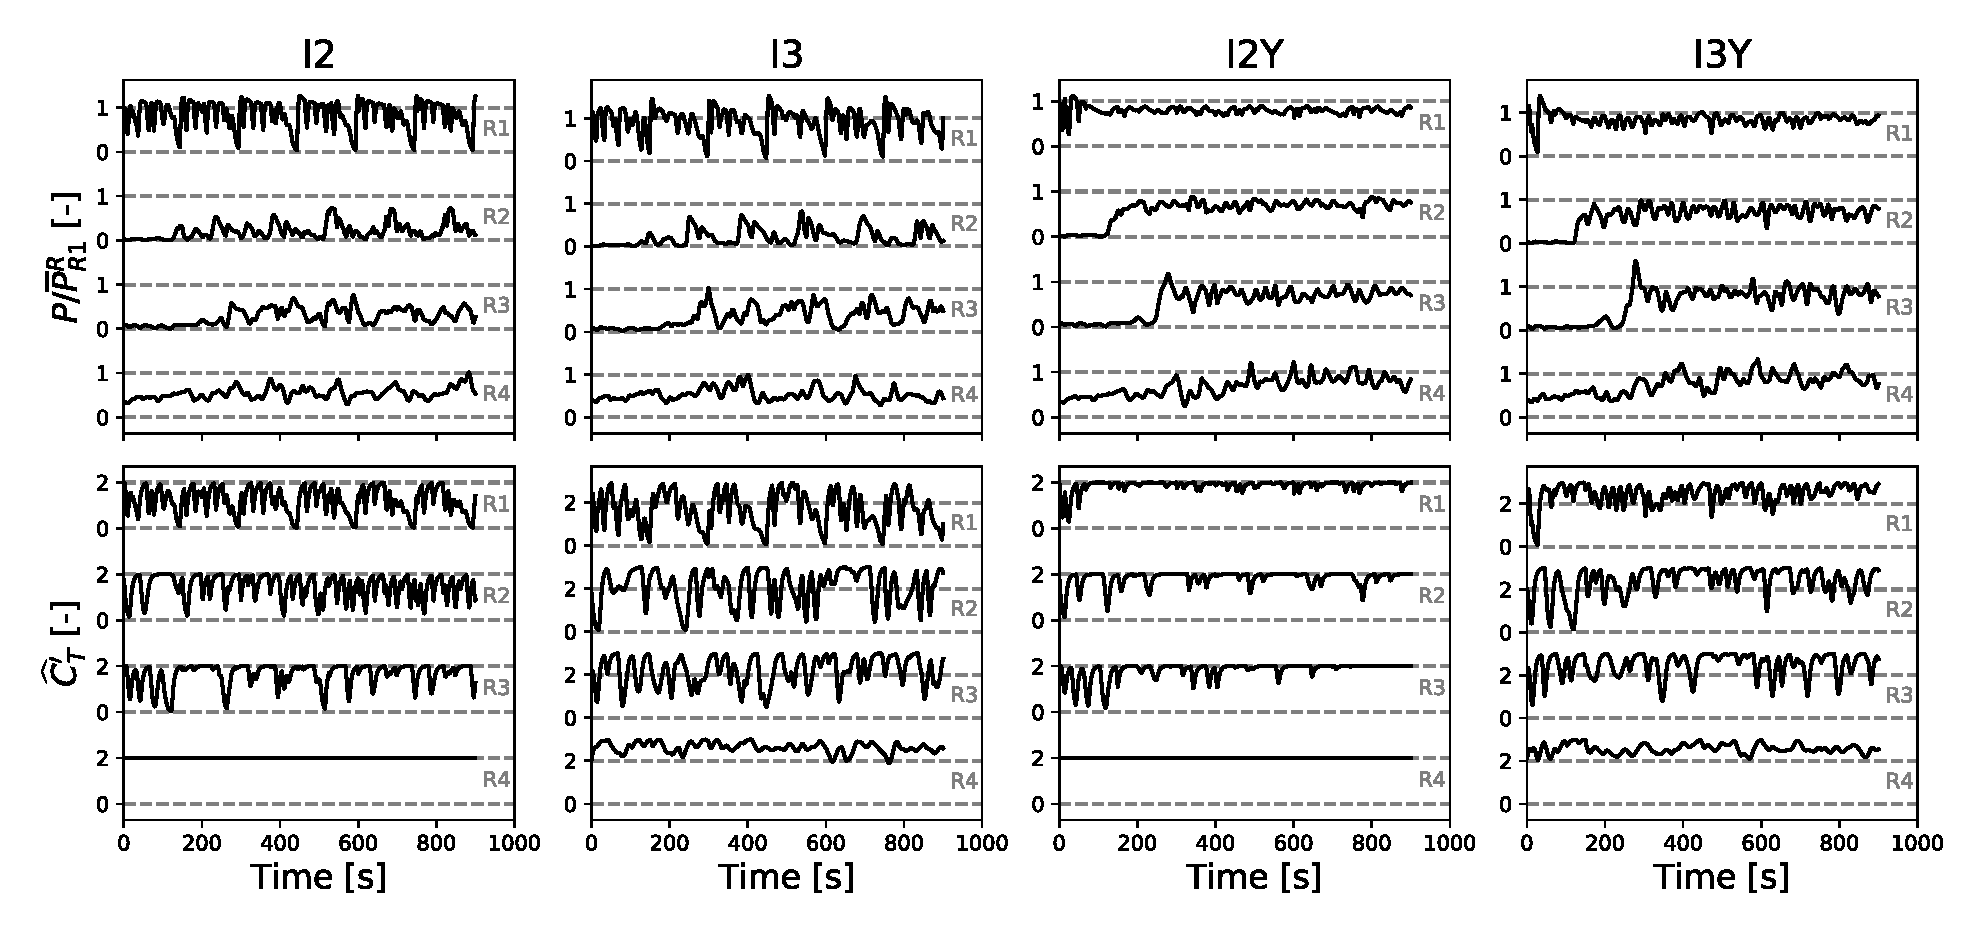
\includegraphics[width=\textwidth]{figure10}	
	\caption{Time evolution of column C1 in uniform inflow induction-enabled cases. \emph{Top: } Turbine power extraction $P$, normalized by mean first row power in the uncontrolled reference $\overline{P}_{R1}^R$. \emph{Bottom: } Thrust coefficient $\widehat{C}_T'$. \label{fig:dynamic_ctfilt}}
\end{figure}

Also the thrust coefficient dynamics vary significantly between different cases: the first-row thrust coefficients of I2 and I3 exhibit periodic oscillatory traits, and the downstream rows of these cases show somewhat more chaotic dynamics in response to unsteady flow conditions resulting from upstream actuation. The period associated with the low-frequency components in the first-row thrust coefficient signal corresponds to the window length, i.e. 150 s, hence indicating that these cases are reacting to finite-horizon effects.  The higher frequencies in this signal are associated with the shedding of vortex rings observed in Figure \ref{fig:flowfield_turb} as discussed above (see also Ref. \cite{muntersphd}).

The underinductive yawing case I2Y features only minor deviations from the reference upper bound value of $\cthat = 2$, especially for $t > 200$ s. This can be explained based on the fact that, after this time, most turbines are yawed with respect to the incoming flow as shown in Figure~\ref{fig:dynamic_uniform}, resulting in a lower axial velocity $V$, and hence a lower thrust force. Further reduction of this thrust force through lower thrust coefficients seems to show only very limited potential in increasing wind-farm power. 

A converse reasoning can be used to explain the induction characteristics in case I3Y: the higher mean values of $\cthat$ in rows 1, 2, and 3 indicate that the wind farm benefits from compensating for the thrust force reduction in yawed turbines by increasing their axial induction. Note that, for the exclusively overinductive case I3, the mean thrust coefficient in the same rows is slightly lower than 2. The last-row turbines of both overinductive cases (I3 and I3Y) are both aligned with the mean flow and show a similar slight increase in the mean thrust coefficient. 

The current section showed results for the \revision{constant} uniform inflow cases. All controlled cases increase wind-farm efficiency by a significant amount, with the yaw-enabled cases significantly outperforming cases based on induction control only. Given the current quiescent ambient flow conditions, simple yaw behavior was identified, i.e. dynamic yaw triggering wake meandering on one hand, and steady yaw resulting in wake redirection on the other hand. Moreover, the simplified control cases Ystat and Ymndr derived from this behavior attain similar wind-farm efficiencies as the optimal control cases. In the next section, unsteady and turbulent inflow conditions are applied, and it is investigated whether similar simplified control methods can be applied.

\subsection{Turbulent inflow}\label{sec:opt_yaw_turb}
\noindent Figure~\ref{fig:flowfield_turb} illustrates snapshots of instantaneous streamwise velocity and wall-normal vorticity at hub height at \revision{t = 300~s} for the reference case R, yawing case Y, overinductive case I3, and combined yaw--overinductive case I3Y. In comparison to the uniform inflow set in Figure~\ref{fig:flowfield_uniform}, the ambient turbulence introduces background vorticity and already destabilizes turbine wakes even in the reference case. Furthermore, wake behavior is much more chaotic and, although traces of wake redirection can be observed for cases Y and I3Y, differences between the flow fields of different cases are far less obvious than in uniform inflow. 
\begin{figure}
	\includegraphics[width=\textwidth]{figure11_revised}
	\caption{Instantaneous planviews at hub height for turbulent inflow cases at \revision{$t= 300$~s}. \emph{Top: } Streamwise velocity. Coloring in m s$^{-1}$. \emph{Bottom: } Wall-normal vorticity. Coloring in s$^{-1}$. \label{fig:flowfield_turb}}
\end{figure}

Similar to the presentation of uniform inflow results in the previous section, firstly power extraction and wind-farm efficiency are illustrated, after which the induction characteristics of inductive cases are shown. Finally, the yaw and power characteristics of the yaw-enabled control cases are described.

\subsubsection{Power extraction and wind-farm efficiency}\label{subsec:turb_powerextr}
\noindent Figure~\ref{fig:power_turb} depicts time-averaged wind-farm power results in the same manner as Figure~\ref{fig:power_uniform}. Figure~\ref{fig:power_turb}a illustrates the row-averaged power extraction for the reference and optimal control cases. Note firstly the much higher power extraction in rows 2 and 3 for the reference case than in the uniform set, caused by the natural destabilization and mixing of turbine wakes by the ambient turbulence. Further, the figure shows that first-row power is being curtailed in all controlled cases. However, for the inductive cases I2 and I3, this curtailment is limited to below 5\%. Significant power gains are achieved in all downstream rows of the inductive cases, except for the second row of I2. For the yaw-enabled cases, curtailment in the first row is smaller than in the uniform inflow set at around 15\%, yet similar flattened power profiles are obtained. 

Figure~\ref{fig:power_turb}b illustrates the wind-farm efficiency for the reference case and the optimal control cases. Similar to the set of uniform inflow cases, also for turbulent inflow two simplified control cases Ystat and Ymndr are defined. These cases are further described and discussed below. A first observation is the higher reference efficiency at 58\% compared to the uniform inflow value of 40\%. Further, the power variability has increased in all cases, as indicated by the wider confidence intervals of the expected values (procedure for calculation of confidence intervals further detailed in Appendix C of Ref. \cite{munters2017optimal}). The exclusively inductive cases I2 and I3 achieve wind-farm efficiencies of 63\% and 67\% respectively. The optimal yaw cases Y, Y5, I2Y, and I3Y attain slightly higher efficiencies of 70\%, 75\%, 73\%, and 78\% respectively. Note that, for unsteady ambient flow conditions, the faster yaw rate in case Y5 significantly increases the efficiency over the standard yaw case~Y. The addition of underinduction control (I2Y) provides a small benefit over standard yaw control (Y), but the highest efficiency is again achieved by overinductive yaw control (I3Y). 

\begin{figure}
	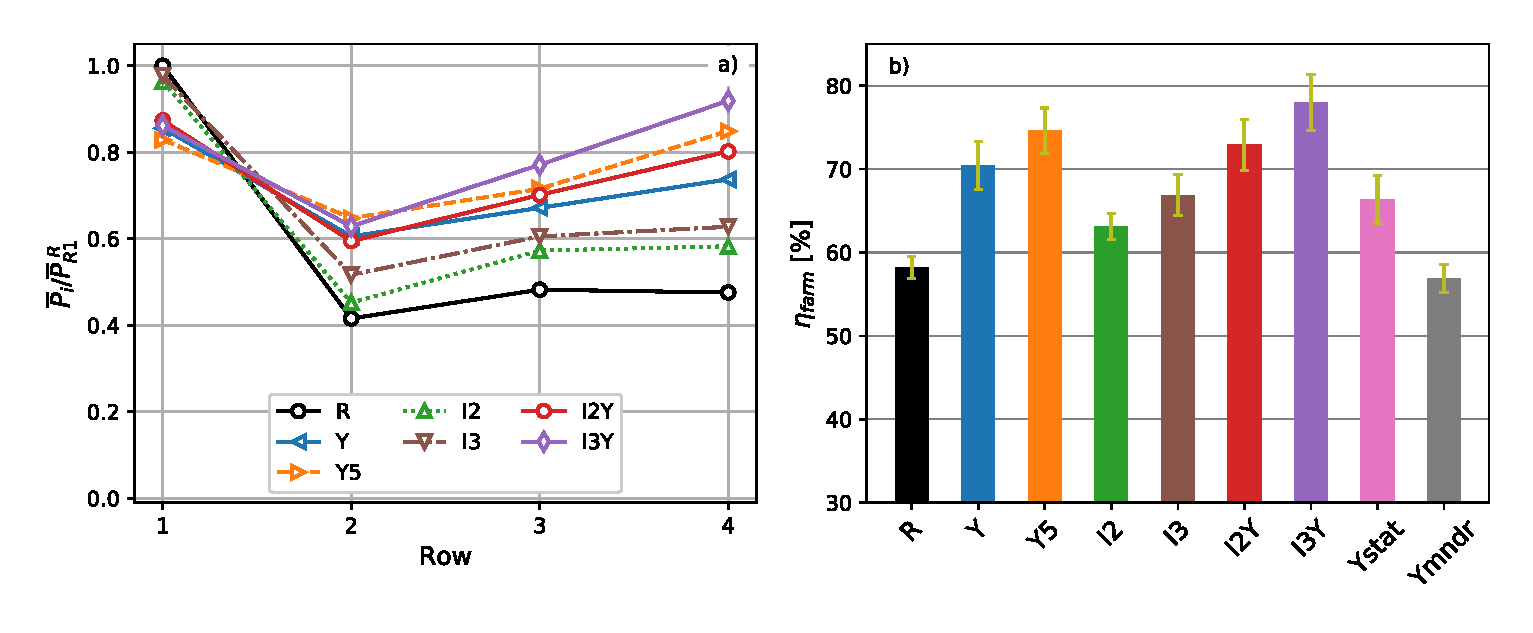
\includegraphics[width=\textwidth]{figure12}
	\caption{\revision{Wind-farm power extraction for reference case R, optimal control cases (Y, Y5, I2, I3, I2Y, and I3Y), and derived control cases (Ystat and Ymndr)}. \emph{a) } Column-averaged power per row, normalized by first-row power of reference case R. \emph{b) } Wind-farm efficiency $\eta_{\text{farm}}$ compared to situation in which all turbines are first-row turbines of R case. Errorbars indicate confidence intervals of $\pm$ 2 standard deviations and are calculated using the procedure detailed in Appendix C of Ref. \cite{munters2017optimal}. \label{fig:power_turb}}
\end{figure}

\subsubsection{Yaw characteristics}\label{subsec:turb_yaw}
\noindent Figure~\ref{fig:dynamic_turb} indicates that both power and yaw angle exhibit significantly more variability compared to the uniform inflow set for all cases. Since wake meandering is already naturally triggered in turbulent boundary layers, the typical wake meandering regime with oscillations around yaw-aligned conditions is not directly observed for any of the cases here. The yaw-enabled cases all seem to turn to the wake redirection regime, characterized by approximately the same yaw angles as in the uniform inflow cases. Note however that there is significant response of the yaw angle to background variability in local flow conditions for all cases, even causing the yaw angle to flip signs sometimes. 
\begin{figure}
	%	\includegraphics[width=\textwidth]{power_angle_ctfilt_lam.eps}
	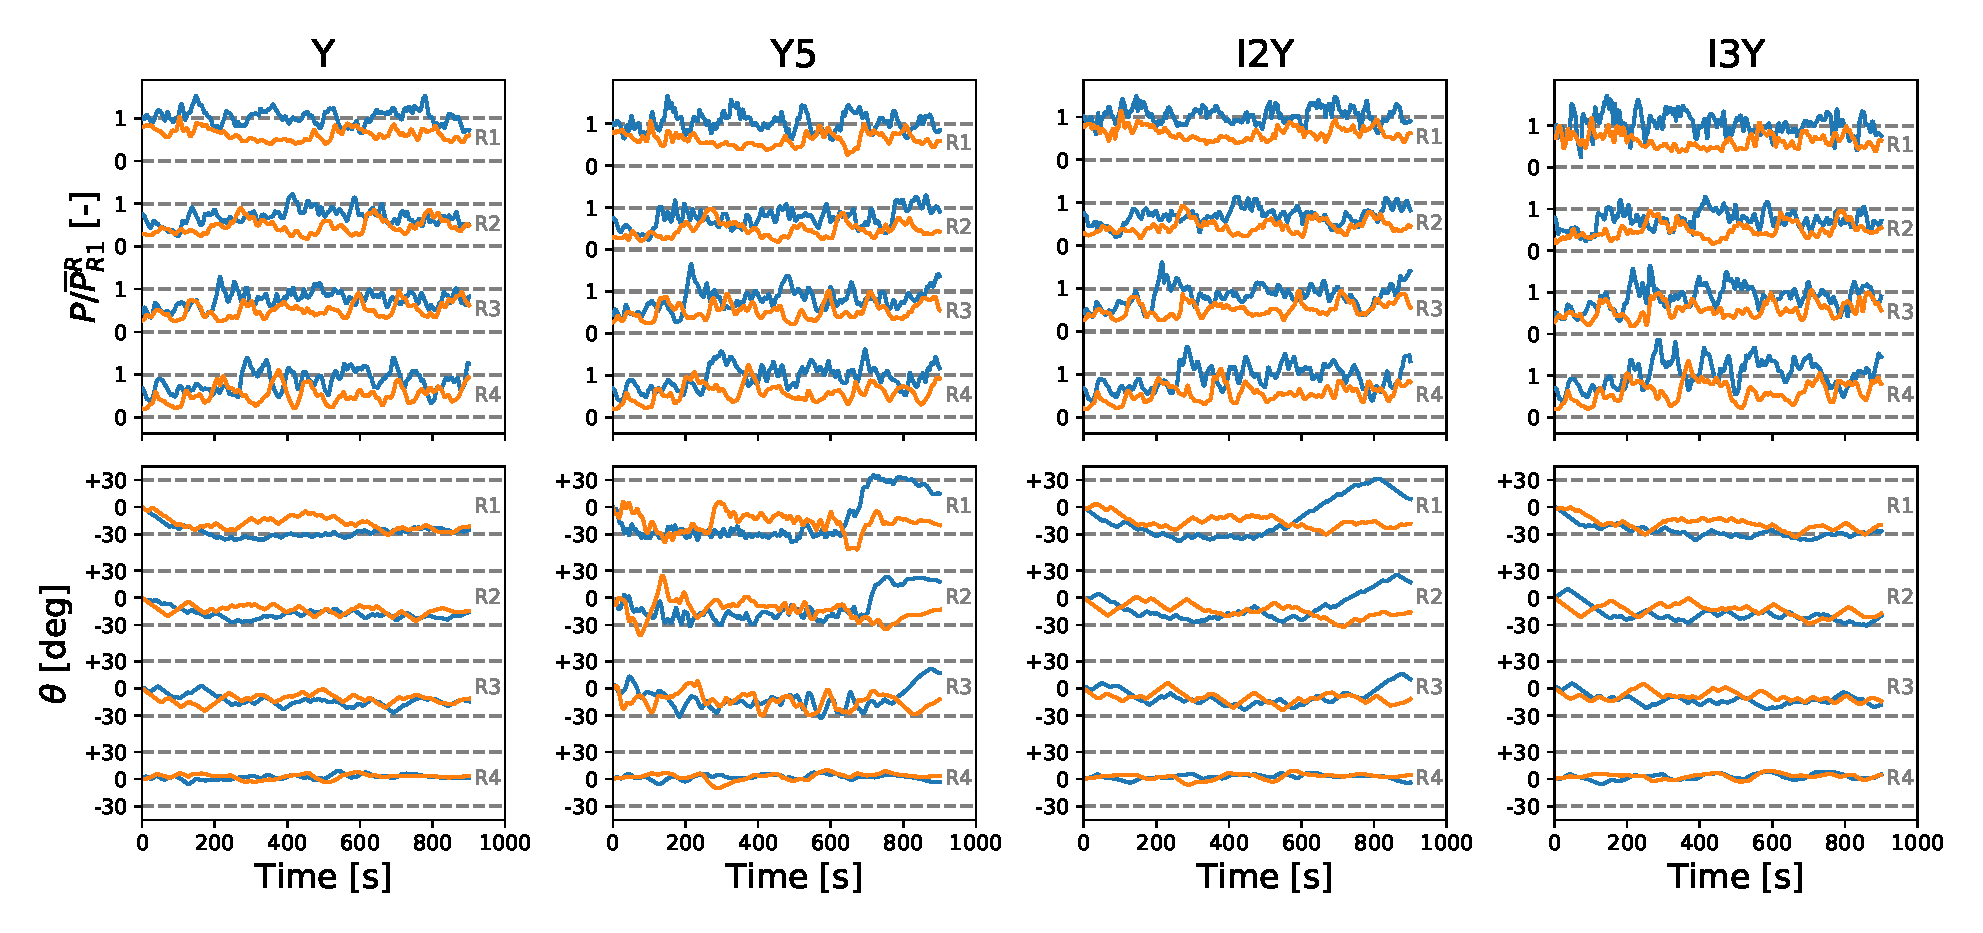
\includegraphics[width=\textwidth]{figure13_revised}	
	\caption{Time evolution of turbulent inflow yaw-enabled cases for columns C2 and C4. \emph{Top: } Turbine power extraction $P$, normalized by mean first row power in the uncontrolled reference $\overline{P}_{R1}^R$. \emph{Bottom: } Yaw angle $\theta$. Line colors indicate different turbine columns {\color{C1} C2}, and {\color{C2} C4} as indicated in Figure~\ref{fig:initial_conditions_flow_yaw}, i.e. every line represents a single wind turbine. \label{fig:dynamic_turb}}
\end{figure}

Figure~\ref{fig:cross_section_turb} illustrates time-averaged cross sections of streamwise velocity $D/2$ upstream of the column C4 turbines for reference case R and yawing case Y. Although wake redirection is complicated by the unsteady inflow, similar deflected and curl-shaped wakes with counter-rotating vortex pairs can be observed for case Y, albeit less explicit than in uniform inflow. Similar characteristics were observed for the other yawing cases Y5, I2Y, and I3Y (not further shown here). Given this information, a similar simplified steady yaw redirection case Ystat was defined, based on the same yaw angles as in the uniform inflow set, i.e. 30$^\circ$, 17$^\circ$, and 17$^\circ$ in rows 1, 2, and 3 respectively. Figure~\ref{fig:power_turb}b illustrates that, although steady yaw control succesfully increases wind-farm efficiency to 66\%, this value is surpassed significantly by the dynamic yawing cases presented above.
\begin{figure}
	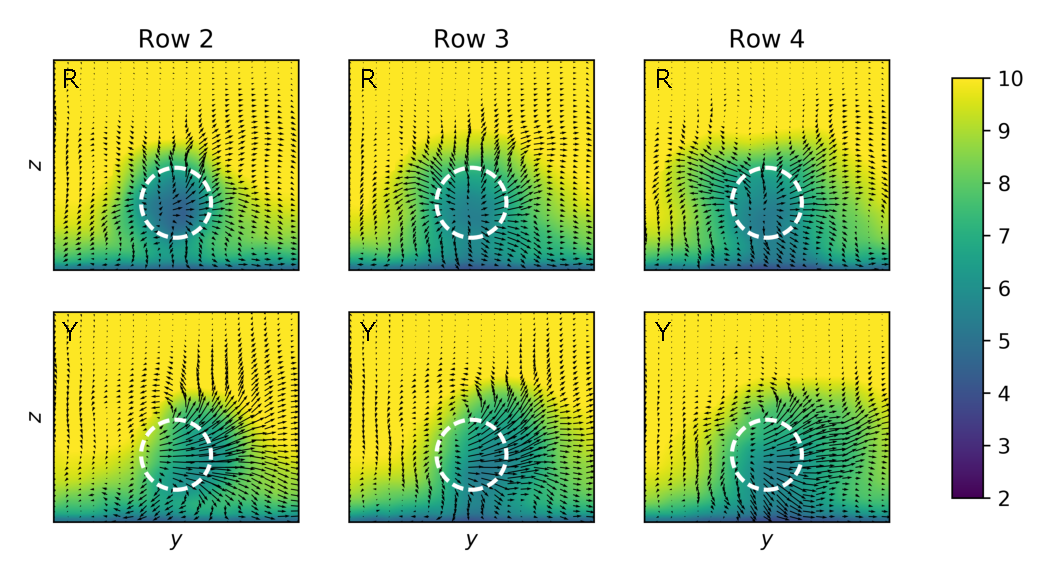
\includegraphics[width=\textwidth]{figure14}
	\caption{Time-averaged cross-sectional views of streamwise velocity $\widetilde{u}_x$ at a distance $D/2$ upstream of the downstream turbines in column C4. Arrows represent the projection of the velocity vector on the cross-sectional plane. Dashed white lines indicate turbine rotor locations. Coloring in m s$^{-1}$. \label{fig:cross_section_turb}}
\end{figure}

Figure~\ref{fig:spec_turbulent} shows the yaw angle power spectral density $S_{\theta \theta}$. Although much less apparent than in the uniform inflow, faint local increases in some of the spectra around $St = 0.2$ can be seen. This raises the suspicion that also in the turbulent inflow case, for which wake meandering is already triggered naturally, the optimizer possibly reinforces meandering through yaw actuation in this frequency range. Therefore, an identical meandering case Ymndr, with bang-bang yaw control at a rate of $\omega = 0.3^\circ$ s$^{-1}$ in the first row was defined. However, Figure~\ref{fig:power_turb}b indicates that this strategy does not lead to an increase in wind-farm efficiency. 
\begin{figure}
	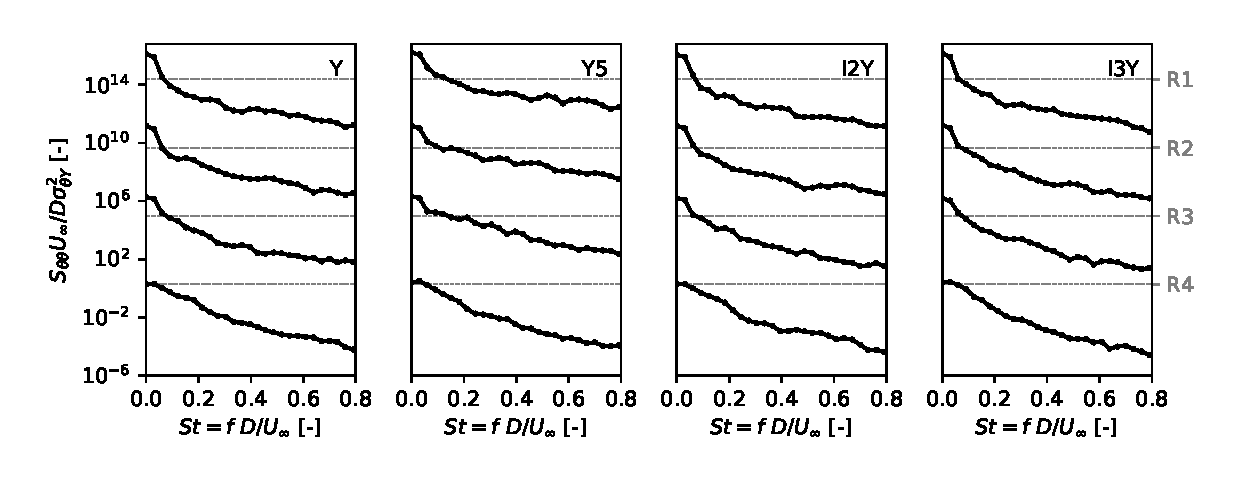
\includegraphics[width=\textwidth]{figure15_revised}
	\caption{\revision{Row-averaged yaw angle power spectral densities $S_{\theta \theta}$ as a function of Strouhal number $St = f D/U_\infty$. Spectra of different rows are shifted vertically for clarity. Horizontal dashed lines indicate identical reference values for each row. Spectra are non-dimensionalized using $\sigma_{\theta Y}^2$, the row-averaged variance of the first row yaw angles in case Y.} \label{fig:spec_turbulent}}
\end{figure}

\subsubsection{Induction characteristics}\label{subsec:turb_induction}
\noindent Figure~\ref{fig:dynamic_ctfilt_turb} depicts the time evolution of power and induction coefficient for the inductive cases I2, I3, I2Y, and I3Y. Similar to the yaw angles described above, also the thrust coefficient appears much more chaotic than in the uniform inflow set, and shows no visually apparent signs of periodic repetitions in control signals. The underinductive cases I2 and I2Y show little deviation from the upper bound. The overinductive cases show similar behavior to the uniform inflow set, i.e. variations around the reference value of $\cthat = 2$ for I3, and a slight increase in mean thrust coefficient for I3Y. 
\begin{figure}
	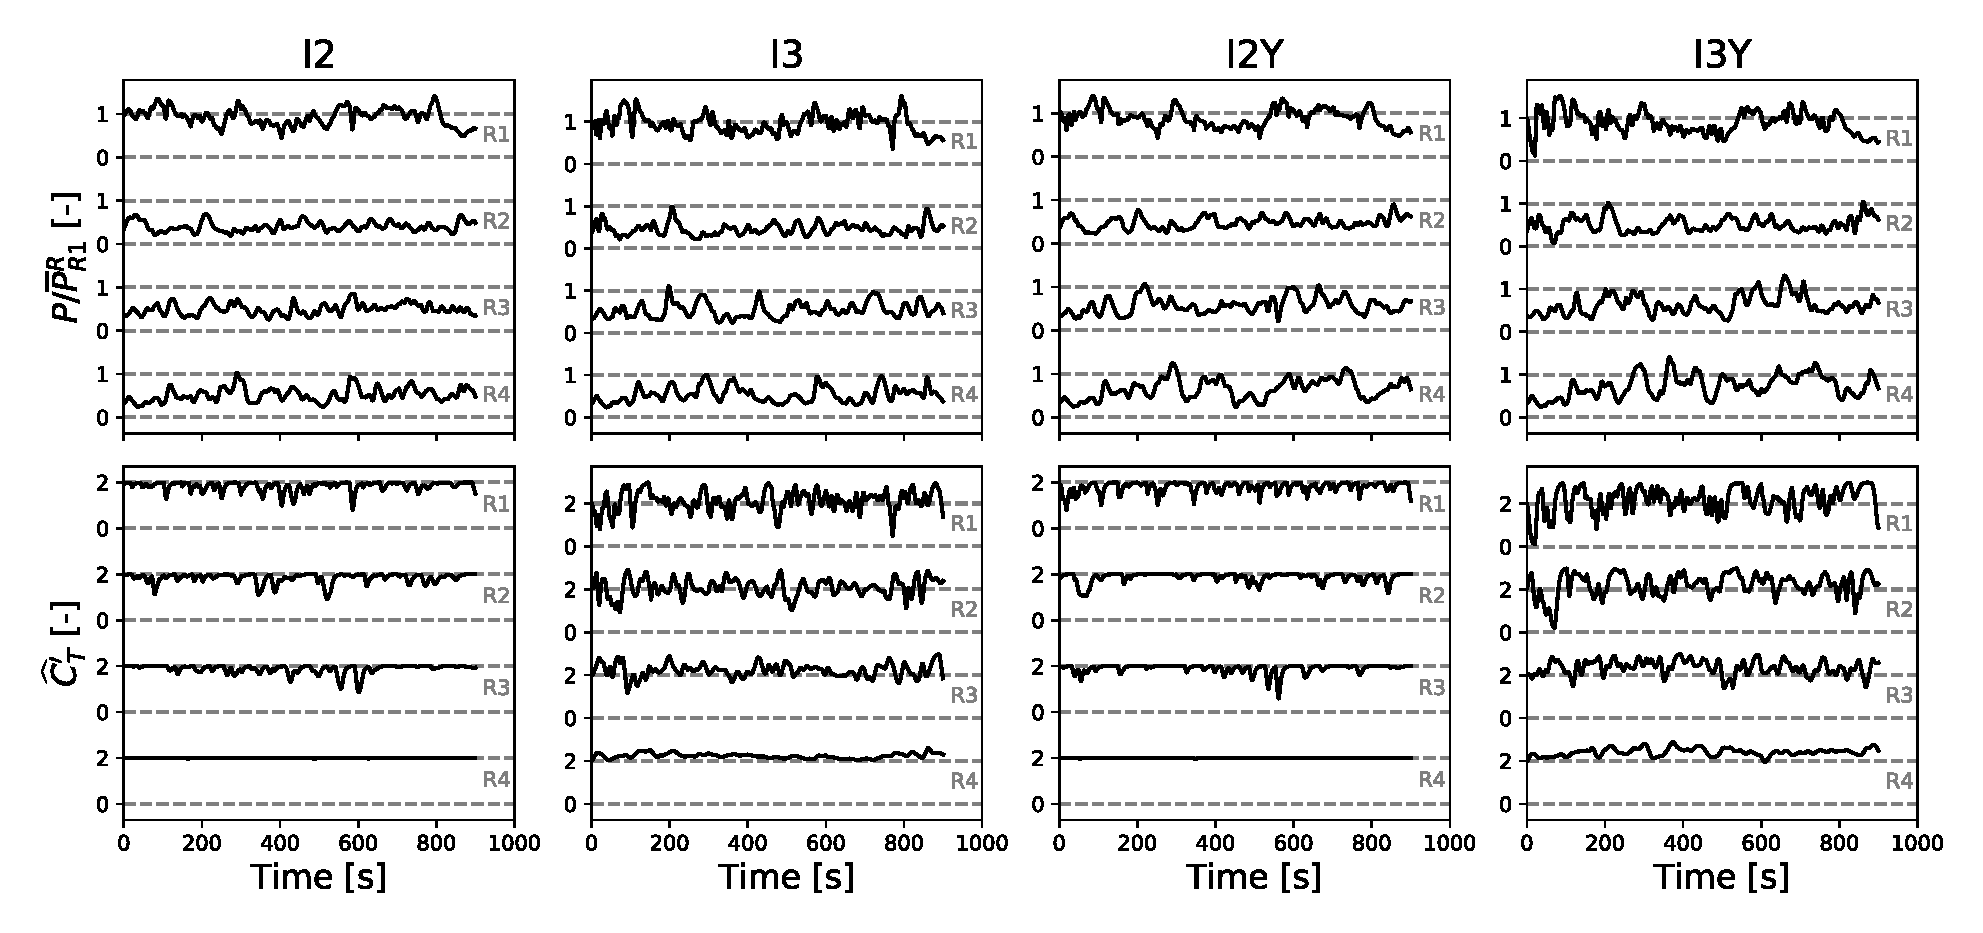
\includegraphics[width=\textwidth]{figure16}	
	\caption{Time evolution of column C1 in turbulent inflow induction-enabled cases. \emph{Top: } Turbine power extraction $P$, normalized by mean first row power in the uncontrolled reference $\overline{P}_{R1}^R$. \emph{Bottom: } Thrust coefficient $\widehat{C}_T'$. \label{fig:dynamic_ctfilt_turb}}
\end{figure}

\subsection{Discussion}\label{sec:opt_yaw_disc}
\begin{table}
	\caption{Summary of wind-farm efficiencies and power gains. Optimal control cases are sorted based on farm efficiency. \label{tab:yaw_summary}}
	\centering
	\begin{tabular}{rlll}
		\toprule
		&   	 & $\eta_{\text{farm}}^{\text{uniform}}$  & $\eta_{\text{farm}}^{\text{turbulent}}$\\
		\midrule
		\multicolumn{1}{l}{\textbf{Greedy control}} & & & \\
		Reference   		    	& R 	 & 0.40					       & 0.58\\
		\\
		\multicolumn{1}{l}{\textbf{Optimal control}} & & & \\
		Underinduction  			& I2 	 & 0.49	[+23\%]				   & 0.63 [+8\%]\\
		Overinduction 	  			& I3 	 & 0.53	[+34\%]				   & 0.67 [+15\%]\\
		Yaw 			    		& Y 	 & 0.77	[+92\%]				   & 0.70 [+21\%]\\
		Underinduction + yaw 		& I2Y 	 & 0.77  [+93\%] 			   & 0.73 [+25\%]\\
		Fast yaw  					& Y5	 & 0.78 [+95\%]  			   & 0.75 [+28\%]\\
		Overinduction + yaw  		& I3Y 	 & 0.84	[+110\%]			   & 0.78 [+34\%]\\
		\\		
		\multicolumn{1}{l}{\textbf{Simplified control}} & & & \\	
		Steady yaw  				& Ystat  & 0.79 	[+97\%]				   & 0.66 [+14\%]\\		        
		Meandering yaw 				& Ymndr  & 0.72 [+79\%] 			   & 0.57 [--2\%]\\					
		\bottomrule
	\end{tabular}
\end{table}

\noindent Table~\ref{tab:yaw_summary} provides an overview of the efficiencies and power gains attained by each of the control cases described in the previous sections. From the table it can be seen that the relative order, based on wind-farm efficiency, is the same for turbulent and uniform inflow conditions. For cases based on exclusively induction control, i.e. I2 and I3, it can be seen that, although the \emph{relative} increase is larger for uniform inflow, the overall attainable wind-farm efficiency is higher for turbulent inflow conditions. 

Further results show that, for the current setup \revision{with a relatively small aligned wind farm}, all yaw-enabled cases consistently outperform cases based solely on axial induction control. However, the gap between both is significantly larger for uniform inflow than for turbulent inflow. The main reason for this is that the yawing cases perform better in the absence of inflow turbulence due to the fact that a \revision{constant incoming} flow allows wakes to be redirected more easily. 

The benefits of combining underinductive axial induction control with yaw control (I2Y) are relatively small: as shown in Figures~\ref{fig:dynamic_uniform} and~\ref{fig:dynamic_turb}, thrust coefficients are barely reduced from their initial upper bound since the thrust forces exerted by turbines in yaw are already reduced through smaller axial velocity components. In contrast, combining overinductive axial induction control with yaw (I3Y) holds much greater promise: in addition to an increase in the mean thrust coefficients, also dynamic thrust variations are observed in Figures~\ref{fig:dynamic_ctfilt} and~\ref{fig:dynamic_ctfilt_turb}, resulting in the highest wind-farm efficiencies obtained for all cases. More specifically, for the current case, Table \ref{tab:yaw_summary} shows that, given turbulent inflow, the gains obtained by overinduction and yaw control are nearly additive, i.e. with a $34\%$ increase for the combined case I3Y, and increases of $21\%$ and $15\%$ for the yawing case Y and overinductive case I3 respectively.

Based on the time evolution of yaw angles in Figures~\ref{fig:dynamic_uniform} and~\ref{fig:dynamic_turb} two simplified cases were defined: a static yaw control case (Ystat) that steadily deflects wakes away from downstream turbines, and a dynamic yaw control case (Ymndr) that imposes an alternating bang-bang control in the first-row turbine to reinforce downstream meandering of the wake. It is important to stress that these are control strategies derived from observations in the optimal control simulations, but no optimization was employed upon generating their control signals. 

The yaw angles used in Ystat, as derived from the dynamic cases, are the same for uniform and turbulent inflow. This indicates that the misalignment angles for steady yaw control are determined by the wind-farm layout geometry, and the dependence on flow conditions is minor. Although Ystat attains virtually identical efficiencies as the dynamic yaw cases Y and Y5 under uniform inflow, its performance under unsteady turbulent flow conditions is surpassed significantly by the latter dynamic cases. This suggests that, in turbulent flows, yaw dynamics play a significant role in increasing wind-farm power in response to continuously changing flow conditions and incident flow angles. This claim is supported by the observation that case Y5 significantly outperforms case Y for turbulent inflow, where this is not true for uniform inflow. 

Further, simplified case Ymndr succeeds in significantly increasing wind-farm efficiency under uniform inflow, and even surpasses the optimization-based induction cases I2 and I3. This is a remarkable result for this very simple control strategy in which active turbines in the first row perform a simple flapping motion, whereas downstream turbines remain passive as in the reference case. However, in turbulent inflow conditions the same strategy did not lead to an increase in power extraction. This can be explained by the fact that meandering is already triggered naturally in turbulent boundary layers. Instead of actively reinforcing downstream wake meandering, the faint traces of spectral peaks at $St = 0.2$ observed in Figure~\ref{fig:spec_turbulent} might therefore simply be the response of yawing turbines to variability in the incident flow angle induced by natural upstream wake meandering. Another hypothesis is that reinforcing natural meandering requires more complex control of the yaw rate than the currently considered bang-bang control, and that the phase of yaw angle variations might have to be matched to local flow conditions. Further research is required to confirm or negate these hypotheses.



\revision{\section{Conclusions and future work}} \label{sec:opt_yaw_concl}
\noindent The current manuscripts investigated the potential of dynamic axial induction and dynamic yaw control for power maximization in an aligned $4 \times 4$ wind farm using large-eddy simulations. A suite of control cases was defined: a set of axial induction control cases with underinductive and overinductive behavior, a set of yaw control cases with standard and high yaw rates, and a set of cases combining induction control with yaw control. For all control cases both uniform and turbulent inflow conditions were considered. In both inflow regimes, yaw control was found to be more effective than induction control for the given wind farm. Furthermore, the significant potential of combining overinduction control with yaw control was shown. Also, distinct regimes in the yaw control cases were identified, a steady yaw wake redirection regime, and a dynamic yawing regime reinforcing wake meandering. Although the former regime was found to be robust to the turbulence levels in the inflow, the latter only achieved an increase in power extraction for uniform conditions. For uniform inflow conditions, it was found that dynamic yawing adds little additional benefit over static wake redirection. In contrast, unsteady yawing allows turbines to adapt to continuously changing local flow conditions, and it was shown that this further increases farm power extraction for turbulent inflow conditions. 

As discussed above, for the given wind-farm setup, yaw control is more favorable than induction control.
An important remark to make is that, as e.g. observed in Figure~\ref{fig:flowfield_uniform} the yawing cases deflect wakes in the transversal direction, and extract energy from the unperturbed flow in the channels between turbine columns. However, in larger wind farms with greater streamwise extent, these channels are naturally depleted of kinetic energy in the downstream regions of the farm due to wake expansion (see for example Ref. \cite{allaerts2017boundary}, Figure 6). As a result, in the downstream regions of very large wind farms, power extraction is governed by vertical transport of kinetic energy \cite{cal2010experimental, calaf2010large}. Furthermore, transversal wake redirection in large yaw-controlled wind farms will lead to wakes interacting with other columns. In contrast, induction control allows for a more isotropic entrainment of kinetic energy, including in the vertical direction. The relative profitability of yaw and induction control is therefore probably dependent on wind-farm size, and turbines might prefer one mechanism over the other depending on their position within the farm. \revision{Moreover, also the wind-farm layout is expected to affect which control mechanism yields more power gains, e.g. the opportunities for wake redirection in aligned wind farms are much better than in staggered wind farms, where deflected wakes will more easily hit turbines in neighboring columns. The question of which control strategy is more effective in larger wind farms with various layouts is subject of current investigation.} 

Further, it is important to note that offshore wind farms typically operate at upstream turbulence intensity (TI) levels of 5--8\%, in between the limit cases of uniform (TI = 0\%) and turbulent inflow (TI = 8\%) considered here \cite{barthelmie2005ten, barthelmie2009modelling}. Moreover, it was already mentioned that in stably stratified boundary layers, turbulence levels are further reduced and wake meandering is suppressed \cite{larsen2009dependence,machefaux2016experimental}. Therefore, the main differences between uniform and turbulent inflow observed here, i.e. the viability of the alternating yawing from Ymndr, and the importance of including dynamic yaw in addition to steady redirection, should be further investigated based on a range of atmospheric conditions for particular wind farms. \revision{Also, throughout this work we considered a constant wind direction and flow forcing. When quantifying potential power gains for real wind farms, the annual distribution of wind speed and velocities at the given site should be taken into account in the flow forcing.} 

\revision{The current optimization studies have been performed using relatively simple non-rotating actuator disk models for the wind turbine rotors without the inclusion of towers or nacelles. Although it has been shown that, by using this approach, the fidelity of far wake characteristics is satisfactory, the credibility of the current power gains and control strategies in practice could be further increased through wind-tunnel testing and similar optimization studies with more detailed turbine models, e.g. by adding drag forces for the tower and nacelle or by representing the rotor with an actuator line model. These are left for future work.} Finally, note that the current study optimizes power at all costs, and did not account for any undesirable loading characteristics. These should also be considered upon thoroughly comparing induction and yaw control for practical purposes. \revision{In this latter case, a detailed turbine representation is of high importance.}











%%%%%%%%%%%%%%%%%%%%%%%%%%%%%%%%%%%%%%%%%%
\vspace{6pt} 

%%%%%%%%%%%%%%%%%%%%%%%%%%%%%%%%%%%%%%%%%%
%% optional
\supplementary{The following are available online at www.mdpi.com/link, Figure S1: title, Table S1: title, Video S1: title.}

%%%%%%%%%%%%%%%%%%%%%%%%%%%%%%%%%%%%%%%%%%
\acknowledgments{The authors acknowledge funding by the European Research Council (ActiveWindFarms, grant no. 306471). The authors also acknowledge support from OPTEC (OPTimization in Engineering Center of Excellence, KU Leuven), which is funded by the KU Leuven Research Council under grant no. PFV/10/002. The computational resources and services in this work were provided by the VSC (Flemish Supercomputer Center), funded by the Research Foundation Flanders (FWO) and the Flemish Government department EWI.}

%%%%%%%%%%%%%%%%%%%%%%%%%%%%%%%%%%%%%%%%%%
\authorcontributions{WM and JM jointly set up the simulation studies in the current work. WM performed code implementations and carried out the simulations. WM and JM jointly wrote the manuscript.}

%%%%%%%%%%%%%%%%%%%%%%%%%%%%%%%%%%%%%%%%%%
\conflictsofinterest{The authors declare no conflict of interest.} 

\appendixtitles{yes} %Leave argument "no" if all appendix headings stay EMPTY (then no dot is printed after "Appendix A"). If the appendix sections contain a heading then change the argument to "yes".
\appendixsections{multiple}
\appendix
\section{Derivation and verification of the adjoint yaw angle equation and the adjoint gradient}\label{sec:app_adj_der}

\noindent In this appendix, we derive the adjoint yaw angle equation in Eq. \ref{eq:adjoint_eta} and the resulting adjoint cost functional gradient in Eq. \ref{eq:problem_gradient}. Furthermore, the continuous adjoint gradient is verified through comparison with a finite difference gradient approximation. 

The derivation of the adjoint equations in this appendix is performed using the formal Lagrangian approach \cite{troltzsch, borzinschulz}, and is elaborated in a similar fashion as in Goit and Meyers \cite{goit2015optimal}. Firstly, inner products and functional gradients are defined in \S\ref{sec:definitions}. Next, the Lagrangian functional for the optimization problem at hand is introduced in \S\ref{sec:define_lagr}. Then, the derivations of the adjoint gradient expression and adjoint yaw angle equation are presented in \S\ref{sec:app_adj_grad} and \S\ref{sec:app_adj_eta} respectively. Finally, the adjoint gradient is verified with a finite-difference gradient approximation in \S\ref{sec:app_adj_verif}. 

\subsection{Definition of inner products and functional gradients}\label{sec:definitions}
\noindent We define inner products between state variables $\bs{q}_1$ and $\bs{q}_2$, and between control variables $\bs{\varphi}_1$ and $\bs{\varphi}_2$ respectively as

\begin{align}
\big( \bs{q}_1, \bs{q}_2 \big) &= \stint \utilde_1 \cdot \utilde_2 ~\dx~\dt + \stint \ptilde_1 \ptilde_2 ~\dx~\dt + \Tint \widehat{\bs{C}}_{T,1}' \cdot \widehat{\bs{C}}_{T,2}' ~\dt+ \Tint \bs{\theta}_1 \cdot \bs{\theta}_2 ~\dt, \\
\big( \bs{\varphi}_1, \bs{\varphi}_2 \big) &= \Tint \bs{C}_{T,1}' \cdot \bs{C}_{T,2}' ~\dt + \Tint \bs{\omega}_1 \cdot \bs{\omega}_2 ~\dt. 
\end{align}

\noindent In these equations, the $\cdot$ operator denotes a dot product between three-dimensional tensor fields, e.g. $\utilde(\bs{x},t) = \big[\widetilde{u}_x(\bs{x},t),\widetilde{u}_y(\bs{x},t),\widetilde{u}_z(\bs{x},t)\big]$, or $N_t$-dimensional vectors, e.g. $\bs{\theta}(t) = \big[\theta_1(t), \dots, \theta_{N_t}(t)\big]$, where appropriate.  In addition, inner products between elements of state and control variables are defined in a similar way, for instance 

\begin{equation}
\big(  \utilde_1, \utilde_2 \big) = \stint \utilde_1 \cdot \utilde_2 ~\dx~\dt, \qquad \text{and} \qquad \big( \bs{\omega}_1 ,\bs{\omega}_2 \big) = \Tint \bs{\omega}_1 \cdot \bs{\omega}_2 ~\dt.
\end{equation}

\noindent The gradient of a differentiable functional is defined as the Riesz representation of its derivative \cite{troltzsch,borzinschulz}. For example, using the definition of the G\^ateaux derivative for a direction $\delta \bs{\varphi}$ in a Hilbert space $\mathscr{\bs{H}}$, the gradient of the reduced cost functional $\nabla \Jtilde$ is defined through

\begin{equation}
\Jtilde_{\bs{\varphi}}(\delta \bs{\varphi}) \equiv \frac{\text{d}}{\text{d}\alpha} \Jtilde (\bs{\varphi}+ \alpha \delta \bs{\varphi}) \bigg\vert_{\alpha=0} = \big( \nabla \Jtilde, \delta \bs{\varphi} \big) = \Tint \nabla \Jtilde \cdot \delta \bs{\varphi} ~\dt \qquad \forall ~\delta \bs{\varphi} \in \mathscr{\bs{H}}
\end{equation}

\subsection{Definition of Lagrangian functional}\label{sec:define_lagr}
\noindent For ease of derivation and notation, we augment the original optimization problem in \eqref{eq:costfunction} with some additional trivial state constraints containing the definitions for the geometric rotor footprint $\R_i$, the rotor-perpendicular vector $\eperpi$, and the rotor disk velocity $V_i$. The box constraints in \eqref{eq:boxct_constraint} -- \eqref{eq:boxomega_constraint} are explicitly taken into account by the L--BFGS--B optimization algorithm, and are omitted in the remainder of the derivation. The resulting augmented optimal control problem hence looks as follows:\footnote{Note that, throughout this text, $\delta [ a ]$ denotes the Dirac delta function applied to a scalar argument $a$, whereas $\delta h$ represents a variation of a functional $h$. }

{\small
\begin{alignat}{4}
& \underset{\bs{\varphi}, \bs{q}}{\text{minimize}}  & \qquad  \J(\bs{\varphi}, \bs{q}) &= - \Tint \sum_{i=1}^{N_t} \frac{1}{2} C_{P,i}'~V_i^3 A_i \dt  & \\
& \text{s.t.}                      			&         \frac{\partial \utilde}{\partial t} + \big(\utilde \cdot \nabla \big)~ \utilde &= - \nabla (\ptilde + \ptilde_\infty) / \rho - \nabla \cdot \boldsymbol{\tau}_{sgs} + \sum_{i=1}^{N_t} - \frac{1}{2} \ctihat~V_i^2 \R_i(\bs{x})~\eperpi \quad  & \text{in } \Omega \times (0,T], \\
&                                                   &        \nabla \cdot \utilde&=0 									        & \text{in } \Omega \times (0,T],\\
&                                                   &        \tau \ddt{\ctihat}&=\cti - \ctihat 								& i=1\dots N_t~\text{in } (0,T],\\
&                                                   &        \ddt{\theta_i}&=\omega_i											& i=1\dots N_t~\text{in } (0,T],\\
&                                                   &        \R_i(\bs{x})&= \sint G(\bs{s} - \bs{x})~H\big[D/2 - \vert\vert \bs{s} - \bs{t}_i \vert\vert_2\big]~\diracdelta \big[ (\bs{s} - \bs{t}_i)\cdot \eperpi \big] \ds											& i=1\dots N_t~\text{in } (0,T], \label{eq:rconstraint}\\
&                                                   &        \eperpi&=\bs{e}_x \cos \theta_i  + \bs{e}_y \sin \theta_i											& i=1\dots N_t~\text{in } (0,T],\\
&                                                   &        V_i&= \vi											& i=1\dots N_t~\text{in } (0,T]. \label{eq:vconstraint}
\end{alignat}
}


\noindent Further, we define the Lagrangian of this optimization problem by adding the state constraints, with shorthand notation $\bs{B}(\bs{\varphi}, \bs{q})$, to the cost functional through inner product with the adjoint variables \revision{$\bs{q}^* = [\bs{\xi}, \pi, \sigma_1, \dots, \sigma_{N_t}, \eta_1, \dots, \eta_{N_t}, \rho_1, \dots, \rho_{N_t}, \bs{\gamma_1}, \dots, \bs{\gamma}_{N_t}, \chi_1, \dots \chi_{N_t}]$, which serve as Lagrange multipliers. The additional variables $\rho_i, \bs{\gamma}_i$, and $\chi_i$ are the adjoint counterparts of $\R_i, \eperpi$, and $V_i$, resulting from including the definitions of the latter as explicit constraints in (\ref{eq:rconstraint} - \ref{eq:vconstraint}). The resulting Lagrangian is expressed as follows:}

\begin{align}
&\mathscr{L}(\bs{\varphi}, \bs{q}, \bs{q}^*) \equiv \J(\bs{\varphi}, \bs{q}) + \innerproduct{\bf{B}(\bs{\varphi}, \bs{q})}{\bs{q}^*} \nonumber\\
&= \Tint \sum_{i=1}^{N_t} - \frac{1}{2} a \ctihat~V_i^3 A_i \dt \nonumber\\
&+ \stint \bigg\{ \frac{\partial \utilde}{\partial t} + \big(\utilde \cdot \nabla \big)~ \utilde + \nabla (\ptilde + \ptilde_\infty) / \rho + \nabla \cdot \boldsymbol{\tau}_{sgs}  - \sum_{i=1}^{N_t} \bs{f}_i \bigg\} \cdot \bs{\xi} \dx \dt \nonumber\\
&+ \stint \bigg\{ \nabla \cdot \utilde \bigg\} \pi \dx \dt \nonumber\\
&+ \Tint \sumturbines \bigg\{  \tau \ddt{\ctihat} - \cti + \ctihat \bigg\} \sigma_i \dt  \nonumber\\
&+ \Tint \sumturbines \bigg\{ \ddt{\theta_i} - \omega_i \bigg\} \eta_i\dt \nonumber\\
&+ \stint \sumturbines \bigg\{ \R_i(\bs{x}) - \sint G(\bs{s} - \bs{x})~H\big[D/2 - \vert\vert \bs{s} - \bs{t}_i \vert\vert_2\big]~\diracdelta \big[ (\bs{s} - \bs{t}_i)\cdot \eperpi \big] \ds \bigg\} \rho_i \dx \dt \nonumber\\
&+ \Tint \sumturbines \bigg\{ \eperpi - \bs{e}_x \cos \theta_i  - \bs{e}_y \sin \theta_i \bigg\} \cdot \bs{\gamma}_i \dt \nonumber \label{eq:lagrangian_derivation}\\
&+ \Tint \sumturbines \bigg\{ V_i - \vi \bigg\} \chi_i \dt .
\end{align}

\noindent The adjoint equations in \eqref{eq:adjoint_momentum} -- \eqref{eq:adjoint_eta} can then be found by postulating vanishing gradients of the Lagrangian as  $\mathscr{L}_{\bs{q}_j}(\delta \bs{q}_j) = (\partial \mathscr{L}/\partial \bs{q}_j, \delta \bs{q}_j) = 0$ with respect to each of the state variables \revision{$\bs{q}_j$ in $\bs{q} = [\utilde, \ptilde, \ctnhat{1}, \dots, \ctnhat{N_t}, \theta_1, \dots, \theta_{N_t}, \R_1, \dots, \R_{N_t}, \eperpn{1}, \dots, \eperpn{N_t}, V_1, \dots, V_{N_t}]$} for all possible variations $\delta \bs{q}_j$ (see, e.g. Refs. \cite{troltzsch,borzinschulz,hinze2008optimization}).  Further, given that these equations are satisfied, the gradient of the reduced cost functional can be found by expressing the sensitivity of the Lagrangian to the control variables as $\Lagr_{\varphi_j}(\delta \varphi_j)$ for the control parameters $\varphi_j$ in $\bs{\varphi} = [\ctn{1}, \dots, \ctn{N_t}, \omega_1, \dots, \omega_{N_t}]$. 
Since the reduced formulation of the optimization problem by definition implies that $B\big(\bs{\varphi}, \bs{q}(\bs{\varphi})\big)=0$, it can be found that the reduced cost functional $\Jtilde$ and the Lagrangian $\Lagr$ are in fact equivalent \cite{hinze2008optimization}, i.e.

\begin{equation}
\Jtilde(\bs{\varphi}) = \Lagr(\bs{\varphi}, \bs{q}(\bs{\varphi}), \bs{q}^*) = \J\big(\bs{\varphi}, \bs{q}(\bs{\varphi})\big) + \innerproduct{\bs{B}\big(\bs{\varphi}, \bs{q}(\bs{\varphi})\big)}{\bs{q}^*}
\end{equation}


\subsection{Derivation of adjoint gradient}\label{sec:app_adj_grad}
\noindent The cost functional gradient $\nabla \Jtilde$ can be found trivially by evaluating the derivative of the Lagrangian in \eqref{eq:lagrangian_derivation} with respect to the thrust setpoints and yaw rate controls as 

\begin{align}
&\Lagr_{\cti}(\delta\cti) = \innerproductsmall{\partial \Lagr /\partial \cti}{\delta \cti} = \big(\partial \Jtilde/\partial \ctihat, \delta \ctihat \big)= \Tint -\sigma_i \ \delta \cti \dt, \label{eq:app_adjoint_grad_sigma}\\
&\Lagr_{\omega_i}(\delta\omega_i) = \innerproductsmall{\partial \Lagr /\partial \omega_i}{\delta \omega_i} =\big( \partial \Jtilde/\partial \omega_i, \delta \omega_i \big)= \Tint -\eta_i \ \delta \omega_i \dt. \label{eq:app_adjoint_grad_eta}
\end{align}

\noindent Hence leading to the gradient expression given in \eqref{eq:problem_gradient}:

\begin{equation}
\nabla \Jtilde \equiv 
\begin{bmatrix*}[l]
\partial \Jtilde / \partial \bs{C}_T' \\
\partial \Jtilde / \partial \bs{\omega} 
\end{bmatrix*} = 
\begin{bmatrix}
- \bs{\sigma}\\
- \bs{\eta}
\end{bmatrix}.
\end{equation}


\subsection{Derivation of adjoint yaw angle equation}\label{sec:app_adj_eta}
\noindent The current section discusses the derivation of the adjoint yaw angle Equation \eqref{eq:adjoint_eta}. To keep notations concise and the derivation clear, we will proceed by first deriving some auxiliary adjoint equations for the rotor footprint $\R_i$ and the disk velocity $V_i$. These will yield straightforward algebraic expressions for the adjoint variables $\rho_i$ and $\chi_i$ respectively, which will be substituted within the derivation of the equation for the adjoint rotor-perpendicular vector $\bs{\gamma}_i$. Thereafter, the adjoint yaw angle equation for the adjoint variable $\eta_i$ will follow in a straightforward manner.

\subsubsection{Adjoint disk velocity equation}
\noindent The adjoint disk velocity equation for the adjoint variable $\chi_i$ is found by expressing the functional derivative of the Lagrangian $\Lagr$ to the disk velocity $V_i$, and equalizing to zero for all possible variations $\delta V_i$, with $i = 1 \dots N_t$: 

\begin{align}
\Lagr_{V_i}(\delta V_i) = \innerproductsmall{\partial \Lagr / \partial V_i}{\delta V_i} &= \Tint -\frac{1}{2} a \ctihat 3 V_i^2 A_i ~\delta V_i ~\dt  + \Tint \frac{1}{2} \ctihat 2 V_i X_i  A_i ~\delta V_i ~\dt + \Tint \chi_i~ \delta V_i ~\dt = 0. 
\end{align}

\noindent This leads to the following expression for the adjoint variable $\chi_i$:

\begin{equation}\label{eq:chi_i}
\chi_i = \frac{1}{2} \ctihat V_i (~3a V_i - 2 X_i )~A_i \qquad\qquad \text{for } i=1\dots N_t. 
\end{equation}

\subsubsection{Adjoint rotor footprint equation}
\noindent The adjoint rotor footprint equation for the adjoint variable $\rho_i$ is found by expressing the derivative of the Lagrangian $\Lagr$ to the footprint $\R_i$: 

\begin{align}
\Lagr_{\R_i}(\delta \R_i) = \stint \frac{1}{2} \ctihat V_i^2 \eperpi \cdot \bs{\xi} ~\delta \R_i ~\dx ~ \dt + \stint \rho_i ~\delta \R_i ~\dx ~\dt + \stint -\frac{\chi_i}{A_i} \utilde \cdot \eperpi ~\delta \R_i ~\dx ~\dt = 0,
\end{align}    

\noindent leading to a straightforward expression of the adjoint variable $\rho_i$:

\begin{align}
\rho_i = \bigg( \frac{\chi_i}{A_i}~\utilde - \frac{1}{2} \ctihat V_i^2 \bs{\xi} \bigg) \cdot \eperpi = \frac{1}{2} \ctihat V_i \bigg(3aV_i \utilde  -2 X_i \utilde - V_i\bs{\xi} \bigg) \cdot \eperpi \qquad\qquad \text{for } i=1\dots N_t. \label{eq:rho_i}
\end{align}

\subsubsection{Adjoint rotor-perpendicular vector equation}
\noindent Similar to the previous sections, the equation for the adjoint rotor-perpendicular vector $\bs{\gamma}_i$ is derived by expressing the derivative of the Lagrangian $\Lagr$ to $\eperpi$:

\begin{align}
\Lagr_{\eperpi}(\delta \eperpi) &= \stint \frac{1}{2} \ctihat V_i^2 \R_i \bs{\xi} \cdot \delta \eperpi \dx ~ \dt - \stint \frac{\chi_i}{A_i} \R_i \utilde \cdot \delta \eperpi \dx~ \dt + \Tint \bs{\gamma}_i \cdot \delta \eperpi \dt \nonumber \\
& + \stint - \rho_i ~ \bigg\{ \sint G(\bs{s} - \bs{x})  H\big[D/2 - \vert\vert \bs{s} - \bs{t}_i \vert\vert_2 \big]~\diracdelta'\big[(\bs{s} - \bs{t}_i) \cdot \eperpi \big]~(\bs{s} - \bs{t}_i) \cdot \delta \eperpi \ds \bigg\} \dx ~\dt \label{eq:app_adj_perp1}.
\end{align}

\noindent The final term in the equation above requires some further attention. The derivative operator on the Dirac delta function can be transferred to the other terms using partial integration by invoking a coordinate transformation from  the LES reference frame $(\bs{e}_x, \bs{e}_y, \bs{e}_z)$ to the rotor reference frame $(\eperpi, \etransi, \bs{e}_z)$, defining a new integration variable $\bs{\zeta} = R\bs{s}$ with $R$ a rotation matrix from the LES to the rotor reference. In doing so, the term between brackets in Equation \eqref{eq:app_adj_perp1} can be rewritten as 

\begin{align}
&\sint G(\bs{s} - \bs{x})  H\big[D/2 - \vert\vert \bs{s} - \bs{t}_i \vert\vert_2 \big]~\frac{\text{d}\diracdelta\big[(\bs{s} - \bs{t}_i) \cdot \eperpi \big]}{\text{d} (\bs{s} - \bs{t}_i) \cdot \eperpi}~(\bs{s} - \bs{t}_i)  \nonumber \ds\\
= &\sint G(\bs{\zeta} - R\bs{x})  H\big[D/2 - \vert\vert \bs{\zeta} - R\bs{t}_i \vert\vert_2 \big]~\frac{\text{d}\diracdelta\big[(\zeta_1 - R\bs{t}_i \cdot \hat{\bs{\zeta}}_1 \big]}{\text{d}\zeta_1}~(\bs{\zeta} - R\bs{t}_i) \dzeta \nonumber \\
= & - \sint \frac{\text{d}}{\text{d}\zeta_1} \bigg\{ G(\bs{\zeta} - R\bs{x})  H\big[D/2 - \vert\vert \bs{\zeta} - R\bs{t}_i \vert\vert_2 \big] (\bs{\zeta} - R\bs{t}_i)  \bigg\} \diracdelta\big[(\zeta_1 - (R\bs{t}_i)_1 \big]~ \dzeta,
\end{align}

\noindent where the boundary terms drop out by the definition of the Dirac delta function. Furthermore, using the chain rule and properties of the Dirac delta function the expression above can be written as 
%\footnote{The term associated with the derivative of the Heaviside function H drops out since it can be rewritten in the form $\int_{-\infty}^{\infty} f(x) x \diracdelta(x)\ \dx$, which vanishes for every bounded function $f(x)$ with compact support.}

\begin{align}
&- \sint \frac{\text{d}}{\text{d}\zeta_1} \bigg\{ G(\bs{\zeta} - R\bs{x})  H\big[D/2 - \vert\vert \bs{\zeta} - R\bs{t}_i \vert\vert_2 \big] (\bs{\zeta} - R\bs{t}_i)  \bigg\} \diracdelta\big[(\zeta_1 - (R\bs{t}_i)_1 \big]~ \dzeta \nonumber\\
&=- \sint G(\bs{\zeta} - R\bs{x})  H\big[D/2 - \vert\vert \bs{\zeta} - R\bs{t}_i \vert\vert_2 \big] \diracdelta\big[(\zeta_1 - (R\bs{t}_i)_1 \big] \bigg\{ \hat{\bs{\zeta}}_1 - \frac{12 \zeta_1 - (R\bs{x})_1}{\Delta^2} (\bs{\zeta} - R \bs{t}_i) \bigg\} ~ \dzeta \nonumber \\
&=- \sint G(\bs{s} - \bs{x})  H\big[D/2 - \vert\vert \bs{s} - \bs{t}_i \vert\vert_2 \big] \diracdelta\big[(\bs{s} - \bs{t})\cdot \eperpi \big] \bigg\{ \eperpi - \frac{12 (\bs{s} - \bs{x})\cdot \eperpi}{\Delta^2} (\bs{s} - \bs{t}_i) \bigg\} ~ \ds.
\end{align}

\noindent Where the last step transforms the coordinate system back to the LES frame of reference. Further, defining the auxiliary variable $\bs{Q}_i = \sint \frac{12 (\bs{s} - \bs{x})\cdot \eperpi}{\Delta^2} (\bs{s} - \bs{t}_i) G(\bs{s} - \bs{x})  H\big[D/2 - \vert\vert \bs{s} - \bs{t}_i \vert\vert_2 \big] \diracdelta\big[(\bs{s} - \bs{t})\cdot \eperpi \big] \ds$ for ease of notation, we find

\begin{align}
\sint G(\bs{s} - \bs{x})  H\big[D/2 - \vert\vert \bs{s} - \bs{t}_i \vert\vert_2 \big]~\diracdelta'\big[(\bs{s} - \bs{t}_i) \cdot \eperpi \big]~(\bs{s} - \bs{t}_i)  \ds 
=  - \R_i \eperpi + \bs{Q}_i. \label{eq:subs_this}
\end{align}

\noindent Substituting expression \eqref{eq:subs_this} into Equation \eqref{eq:app_adj_perp1}, along with the expressions for $\rho_i$ (Equation \ref{eq:rho_i}) and $\chi_i$ (Equation \ref{eq:chi_i}) yields:

\begin{align}
\Lagr_{\eperpi}(\delta \eperpi) &= - \stint \frac{1}{2} \ctihat V_i \bigg\{ 3a V_i \utilde  - 2 X_i \utilde - V_i\bs{\xi}   \bigg\} \R_i \cdot \delta \eperpi \dx \dt + \Tint \bs{\gamma}_i \cdot \delta \eperpi \dt \nonumber\\
& + \stint \frac{1}{2} \ctihat V_i \bigg\{ \bigg(3aV_i \utilde  -2 X_i \utilde - V_i\bs{\xi} \bigg) \cdot \eperpi \bigg\} \R_i \eperpi \cdot \delta \eperpi \ds \nonumber \\
& - \stint \frac{1}{2} \ctihat V_i \bigg\{ \bigg(3aV_i \utilde  -2 X_i \utilde - V_i\bs{\xi} \bigg) \cdot \eperpi \bigg\} \bs{Q}_i \cdot \delta \eperpi \ds. 
\end{align}

\noindent Since there is no rotor tilt, it can be seen that $\bs{v} - ( \bs{v} \cdot \eperpi ) \eperpi = (\bs{v} \cdot \etransi) \etransi$, for any vector $\bs{v}$ in $\Omega \times (0, T]$. Hence, 

\begin{align}
\Lagr_{\eperpi}(\delta \eperpi) &= \Tint \bs{\gamma}_i \cdot \delta \eperpi \dt \nonumber\\
& - \stint \frac{1}{2} \ctihat V_i \bigg\{ \bigg(3a V_i \utilde  - 2 X_i \utilde - V_i\bs{\xi} \bigg) \cdot \etransi   \bigg\} \R_i \etransi \cdot \delta \eperpi \dx \dt \nonumber \\
& - \stint \frac{1}{2} \ctihat V_i \bigg\{ \bigg(3aV_i \utilde  -2 X_i \utilde - V_i\bs{\xi} \bigg) \cdot \eperpi \bigg\} \bs{Q}_i \cdot \delta \eperpi \ds 
\end{align}

\noindent Equating to zero finally yields the expression for the adjoint rotor-perpendicular vector $\bs{\gamma}_i$:

\begin{align}
\bs{\gamma}_i = \frac{1}{2} \ctihat V_i \sint \bigg[ & \bigg\{ \bigg(3a V_i \utilde  - 2 X_i \utilde - V_i\bs{\xi} \bigg) \cdot \etransi   \bigg\} \R_i \etransi + \bigg\{ \bigg(3aV_i \utilde  -2 X_i \utilde - V_i\bs{\xi} \bigg) \cdot \eperpi \bigg\} \bs{Q}_i \bigg] \ds. \label{eq:app_adj_gamma_final}  
\end{align}

\subsubsection{Adjoint yaw angle equation}
\noindent The current section derives the adjoint equation for the adjoint yaw angle $\eta_i$, required for the evaluation of the cost functional yaw sensitivity in Equation \eqref{eq:app_adjoint_grad_eta}. Similar to previous sections, the derivation starts by expressing the functional derivative of the Lagrangian to the yaw angle $\theta_i$: 

\begin{align}
\Lagr_{\theta_i}(\delta \theta_i) &= 
\Tint \bs{\gamma}_i \cdot \bigg\{ \bs{e}_x \sin \theta_i - \bs{e}_y \cos \theta_i  \bigg\} \delta \theta_i ~\dt + \Tint \ddt{\delta \theta_i} \eta_i ~\dt \\ 
&= \Tint \bigg\{ -\ddt{\eta_i} - \etransi \cdot \bs{\gamma}_i   \bigg\} \delta \theta_i \dt = 0,
\end{align}

\noindent Where partial integration on the time derivative is performed, and a terminal condition $\eta_i(T) = 0$ is applied, leading to vanishing boundary terms. This yields an ODE for $\eta_i$:

\begin{equation}\label{eq:app_adj_eta_basic}
- \ddt{\eta_i} = \bs{e}_{\parallel,i} \cdot \bs{\gamma}_i 
\qquad\qquad \text{for } i=1\dots N_t.
\end{equation}

\noindent Substituting the expression for $\bs{\gamma}_i$ from Equation \eqref{eq:app_adj_gamma_final}, this expression can be rewritten as 

\begin{align}
- \ddt{\eta_i} =  \frac{1}{2} \ctihat V_i \sint \bigg[ & \bigg\{ \bigg(3a V_i \utilde  - 2 X_i \utilde - V_i\bs{\xi} \bigg) \cdot \etransi   \bigg\} \R_i + \bigg\{ \bigg(3aV_i \utilde  -2 X_i \utilde - V_i\bs{\xi} \bigg) \cdot \eperpi \bigg\} \mathscr{Q}_i \bigg] \ds, \label{eq:app_adj_eta_final} 
\end{align}

\noindent which is the adjoint equation for $\eta_i$ featured in Equation \eqref{eq:adjoint_eta}. In this equation, the shorthand notation for the filter kernel $\mathscr{Q}_i$ is introduced as:

\begin{align}
\mathscr{Q}_i = \bs{Q}_i \cdot \etransi = \sint \frac{12 (\bs{s} - \bs{x})\cdot \eperpi}{\Delta^2} G(\bs{s} - \bs{x})  H\big[D/2 - \vert\vert \bs{s} - \bs{t}_i \vert\vert_2 \big] \diracdelta\big[(\bs{s} - \bs{t})\cdot \eperpi \big]  (\bs{s} - \bs{t}_i) \cdot \etransi \ds.
\end{align}

\noindent Figure \ref{fig:filters} illustrates both the original filter kernel $\R$ and the new filter kernel $\mathscr{Q}_i$. It can be seen from the figure that $\mathscr{Q}_i$ quantifies the rate of change in the rotor geometrical footprint $\R_i$ upon perturbing the yaw angle $\theta$. Therefore, $\mathscr{Q}_i$ can be regarded as a yaw-sensitivity footprint.
Further, given Equation \eqref{eq:app_adjoint_grad_eta}, it can be seen that the right-hand-side of Equation \eqref{eq:app_adj_eta_final} acts as a driving term for the yaw rate sensitivity. The first term in the right-hand-side is associated with the flow currently parallel to the rotor, which is hence not captured given its current orientation, imposing an incentive for reorientation of the rotor. The second on the other hand is associated with the flow perpendicular to the rotor just before or behind the rotor plane. This term causes an incentive for yawing since a change in rotor locus (i.e. where the flow field is sampled by the ADM) would allow power to be extracted from these terms. 

\begin{figure}
	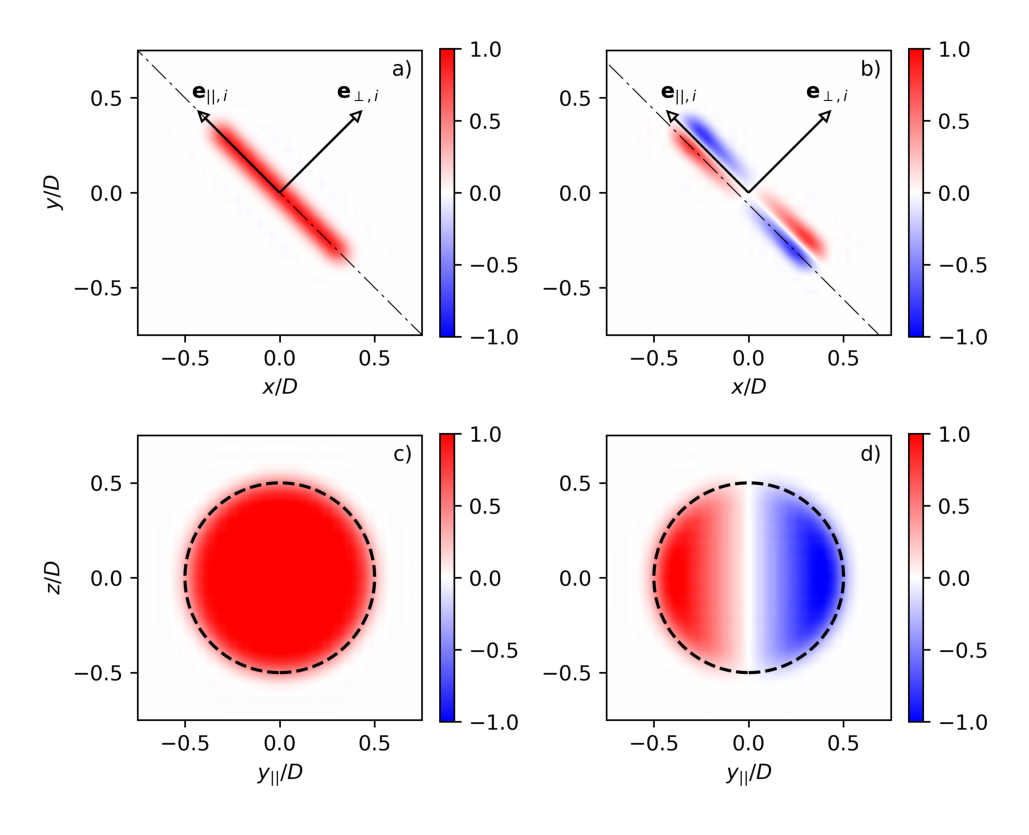
\includegraphics[width=\textwidth]{figure17}
	\caption{Geometrical filter kernels in Equation \eqref{eq:app_adj_eta_final}. \emph{a,c)} Original stationary rotor footprint $\R$. \emph{b,d)} New yaw-sensitivity footprint $\mathscr{Q}$. \emph{a,b)} Planview at hub height. \emph{c,d)} Cross section through plane indicated by dot dashed line in \emph{a},\emph{b}. \label{fig:filters}}
\end{figure}

\subsection{Verification of adjoint gradient}\label{sec:app_adj_verif}
\noindent The current section aims to verify the continuous adjoint method applied in this manuscript through comparison with a finite-difference approximation of the cost functional gradient. Since the accuracy of the continuous adjoint method is dependent on the spatiotemporal resolution with which the equations are discretized, the test is performed on a case with identical resolution as the cases defined in the main text. To limit computational cost, a domain of reduced size with only 2 aligned turbines is considered. The simulation domain of $2.4 \times 0.6 \times 0.5$ km$^3$ is discretized on a grid of $128 \times 32 \times 64$, resulting in a grid resolution of $18.75 \times 18.75 \times 7.8$ m$^3$ simulated over a time horizon of 300 s with time steps of 0.75 s, identical to the simulations in the main text (see Table \ref{tab:case_definition}).

The finite difference method approximates the G\^ateaux derivative in a direction $\delta \bs{\varphi}$ as

\begin{equation}\label{eq:finitediff_grad}
\innerproduct{\nabla \Jtilde}{\delta \bs{\varphi}} \approx \frac{\Jtilde(\bs{\varphi} + \alpha \delta \bs{\varphi}) - \Jtilde(\bs{\varphi})}{\alpha},
\end{equation}

\noindent where $\alpha$ is sufficiently small yet large enough to avoid round-off errors due to finite-precision floating-point arithmetic. In the current work, $\alpha$ is chosen such that control perturbations are five orders of magnitude smaller than baseline controls. Approximating the full gradient $\nabla \Jtilde$ would require evaluating Equation \eqref{eq:finitediff_grad} for as many linearly independent directions $\delta \bs{\varphi}$ as there are dimensions in $\bs{\varphi}$. Here, we only evaluate a limited amount of gradient components, by choosing a set of pointwise unit perturbations $\delta \varphi_i(t^*)$ to the baseline controls of each of the turbines $i$ at different times $t^*$. 

Figure~\ref{fig:forwardfield_adjointfield} illustrates snapshots of both the forward and adjoint solutions at hub height. From Figure~\ref{fig:forwardfield_adjointfield}b it can be seen that the adjoint field starts out as streamtubes from the turbines indicating where immediate changes in the cost function originate, and transitions to a chaotic field after some upstream distance. 

\begin{figure}[ht]
	\centering
	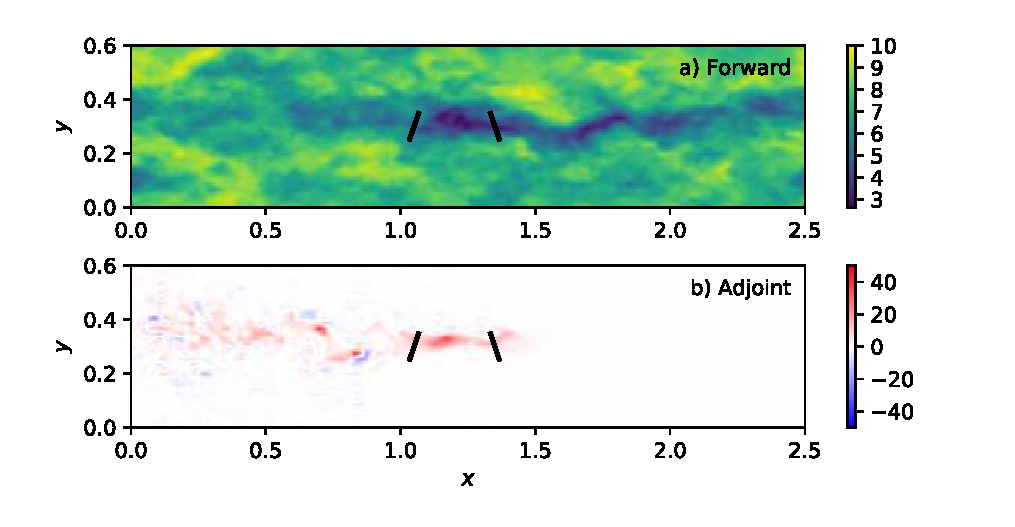
\includegraphics[width=0.9\textwidth]{figure18}
	\caption{Solution fields for adjoint gradient verification test case at $t=150$ s. \emph{a)} Forward field $\tilde{u}_x$. \emph{b)} Adjoint field $\xi_x$. \label{fig:forwardfield_adjointfield}}
\end{figure}

\begin{figure}[h!]
	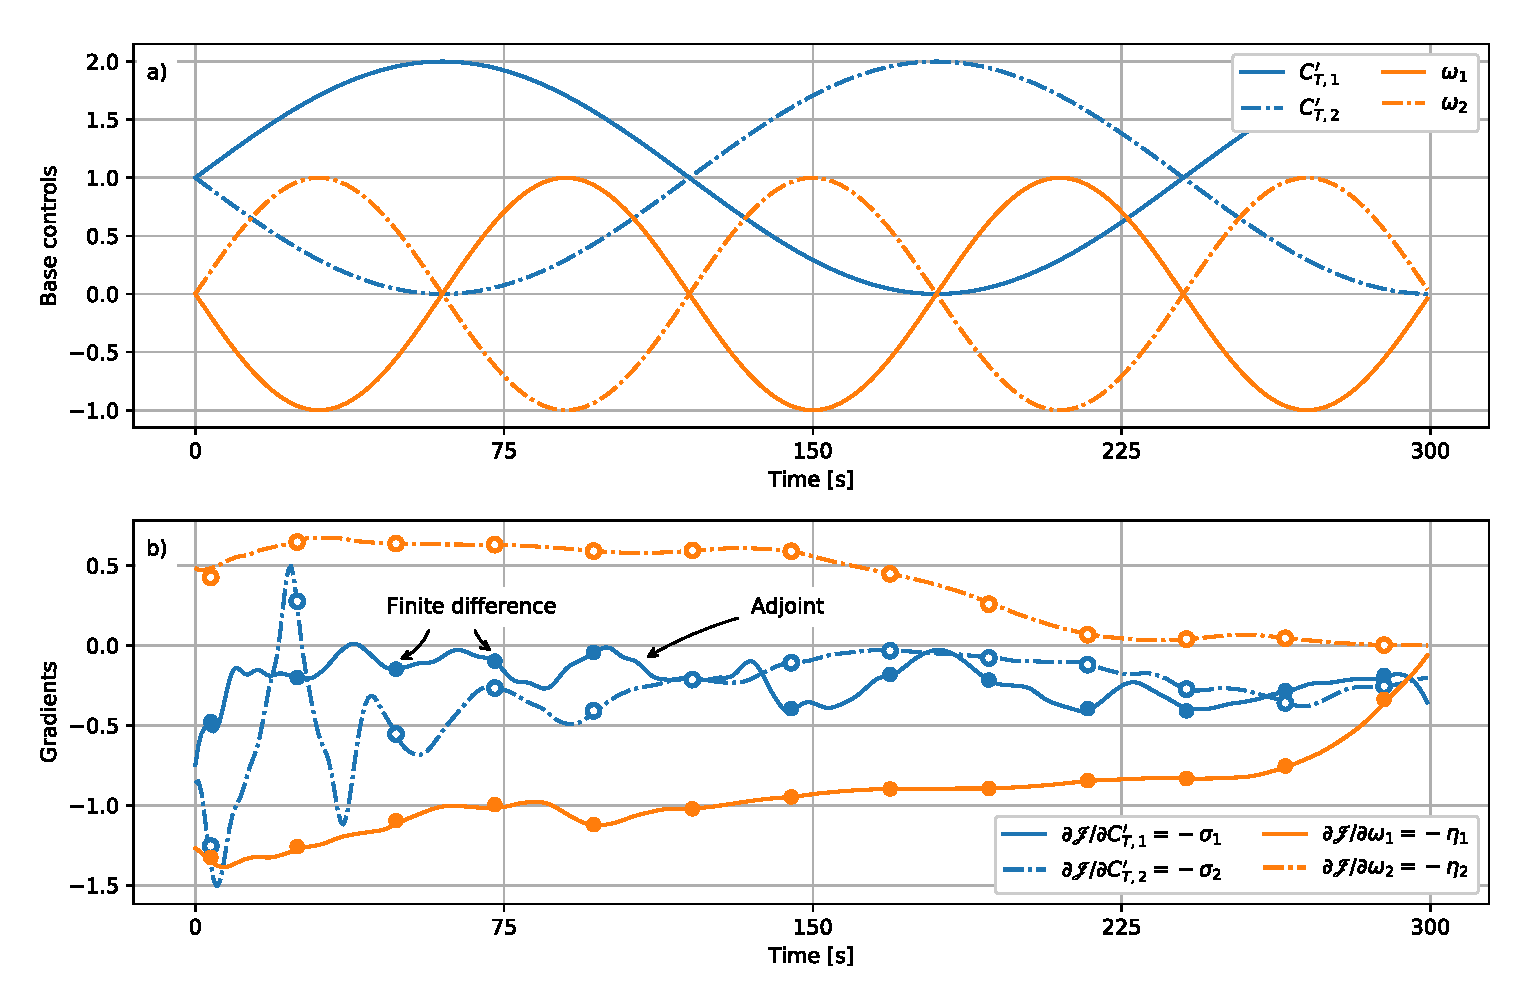
\includegraphics[width=\textwidth]{figure19}
	\caption{Adjoint gradient verification case. \emph{a)} Baseline controls around which linearization is performed. \emph{b)} Cost functional gradient. Full lines: adjoint, dots: finite-difference. \label{fig:gradient_verification}}
\end{figure}

Figure~\ref{fig:gradient_verification} illustrates the baseline controls $\bs{\varphi}$ around which the linearization is performed (Fig. \ref{fig:gradient_verification}a), as well as the adjoint gradient (full lines) compared to the finite difference gradient component approximations (dots) described above (Fig. \ref{fig:gradient_verification}b). It can be seen from the figure that the gradient approximations match well. The overall relative error between both remains below 5$\%$. Note that, although this error could be further reduced through grid refinement, the current gradient accuracy is adequate for the optimizations considered in this work.

\reftitle{References}
\begin{thebibliography}{999}
	\providecommand{\natexlab}[1]{#1}
	
	\bibitem[Boersma \em{et~al.}(2017)Boersma, Doekemeijer, Gebraad, Fleming,
	Annoni, Scholbrock, Frederik, and van Wingerden]{boersma2017tutorial}
	Boersma, S.; Doekemeijer, B.; Gebraad, P.; Fleming, P.; Annoni, J.; Scholbrock,
	A.; Frederik, J.; van Wingerden, J.
	\newblock A tutorial on control-oriented modeling and control of wind farms.
	\newblock  American Control Conference (ACC), 2017. IEEE,  2017, pp. 1--18.
	
	\bibitem[Knudsen \em{et~al.}(2015)Knudsen, Bak, and
	Svenstrup]{knudsen2015survey}
	Knudsen, T.; Bak, T.; Svenstrup, M.
	\newblock Survey of wind farm control - power and fatigue optimization.
	\newblock {\em Wind Energy} {\bf 2015}, {\em 18},~1333--1351.
	
	\bibitem[Annoni \em{et~al.}(2016)Annoni, Gebraad, Scholbrock, Fleming, and
	Wingerden]{annoni2016analysis}
	Annoni, J.; Gebraad, P.M.O.; Scholbrock, A.K.; Fleming, P.A.; Wingerden, J.W.v.
	\newblock Analysis of axial-induction-based wind plant control using an
	engineering and a high-order wind plant model.
	\newblock {\em Wind Energy} {\bf 2016}, {\em 19},~1135--1150.
	\newblock we.1891.
	
	\bibitem[Steinbuch \em{et~al.}(1988)Steinbuch, de~Boer, Bosgra, Peters, and
	Ploeg]{steinbuch}
	Steinbuch, M.; de~Boer, W.; Bosgra, O.; Peters, S.; Ploeg, J.
	\newblock Optimal control of wind power plants.
	\newblock {\em Journal of Wind Engineering and Industrial Aerodynamics} {\bf
		1988}, {\em 27},~237 -- 246.
	
	\bibitem[Horvat \em{et~al.}(2012)Horvat, Spudi{\'c}, and
	Baoti{\'c}]{horvat2012quasi}
	Horvat, T.; Spudi{\'c}, V.; Baoti{\'c}, M.
	\newblock Quasi-stationary optimal control for wind farm with closely spaced
	turbines.
	\newblock  MIPRO, 2012 Proceedings of the 35th International Convention. IEEE,
	2012, pp. 829--834.
	
	\bibitem[Johnson and Fritsch(2012)]{johnson2012assessment}
	Johnson, K.E.; Fritsch, G.
	\newblock Assessment of extremum seeking control for wind farm energy
	production.
	\newblock {\em Wind Engineering} {\bf 2012}, {\em 36},~701--715.
	
	\bibitem[Gebraad and Van~Wingerden(2015)]{gebraad2015maximum}
	Gebraad, P.; Van~Wingerden, J.
	\newblock Maximum power-point tracking control for wind farms.
	\newblock {\em Wind Energy} {\bf 2015}, {\em 18},~429--447.
	
	\bibitem[Nilsson \em{et~al.}(2015)Nilsson, Ivanell, Hansen, Mikkelsen,
	S{\o}rensen, Breton, and Henningson]{nilsson2015large}
	Nilsson, K.; Ivanell, S.; Hansen, K.S.; Mikkelsen, R.; S{\o}rensen, J.N.;
	Breton, S.P.; Henningson, D.
	\newblock Large-eddy simulations of the Lillgrund wind farm.
	\newblock {\em Wind Energy} {\bf 2015}, {\em 18},~449--467.
	
	\bibitem[Campagnolo \em{et~al.}(2016)Campagnolo, Petrovi{\'c}, Bottasso, and
	Croce]{campagnolo2016wind}
	Campagnolo, F.; Petrovi{\'c}, V.; Bottasso, C.L.; Croce, A.
	\newblock Wind tunnel testing of wake control strategies.
	\newblock  American Control Conference (ACC), 2016. IEEE,  2016, pp. 513--518.
	
	\bibitem[Bartl and S{\ae}tran(2016)]{bartl2016experimental}
	Bartl, J.; S{\ae}tran, L.
	\newblock Experimental testing of axial induction based control strategies for
	wake control and wind farm optimization.
	\newblock {\em Journal of Physics: Conference Series} {\bf 2016}, {\em
		753},~032035.
	
	\bibitem[Goit and Meyers(2015)]{goit2015optimal}
	Goit, J.P.; Meyers, J.
	\newblock Optimal control of energy extraction in wind-farm boundary layers.
	\newblock {\em J Fluid Mech} {\bf 2015}, {\em 768},~5--50.
	
	\bibitem[Goit \em{et~al.}(2016)Goit, Munters, and Meyers]{goit2016optimal}
	Goit, J.P.; Munters, W.; Meyers, J.
	\newblock Optimal Coordinated Control of Power Extraction in {LES} of a Wind
	Farm with Entrance Effects.
	\newblock {\em Energies} {\bf 2016}, {\em 9},~29.
	
	\bibitem[Munters and Meyers(2016)]{munters2016effect}
	Munters, W.; Meyers, J.
	\newblock Effect of wind turbine response time on optimal dynamic induction
	control of wind farms.
	\newblock {\em Journal of Physics: Conference Series} {\bf 2016}, {\em
		753},~052007.
	
	\bibitem[Munters and Meyers(2017)]{munters2017optimal}
	Munters, W.; Meyers, J.
	\newblock An optimal control framework for dynamic induction control of wind
	farms and their interaction with the atmospheric boundary layer.
	\newblock {\em Philos T Roy Soc A} {\bf 2017}.
	
	\bibitem[Fleming \em{et~al.}(2014)Fleming, Gebraad, Lee, van Wingerden,
	Johnson, Churchfield, Michalakes, Spalart, and
	Moriarty]{fleming2014evaluating}
	Fleming, P.A.; Gebraad, P.M.; Lee, S.; van Wingerden, J.W.; Johnson, K.;
	Churchfield, M.; Michalakes, J.; Spalart, P.; Moriarty, P.
	\newblock Evaluating techniques for redirecting turbine wakes using SOWFA.
	\newblock {\em Renewable Energy} {\bf 2014}, {\em 70},~211--218.
	
	\bibitem[Bossanyi(2003)]{bossanyi2003individual}
	Bossanyi, E.
	\newblock Individual blade pitch control for load reduction.
	\newblock {\em Wind energy} {\bf 2003}, {\em 6},~119--128.
	
	\bibitem[Fleming \em{et~al.}(2015)Fleming, Gebraad, Lee, van Wingerden,
	Johnson, Churchfield, Michalakes, Spalart, and
	Moriarty]{fleming2015simulation}
	Fleming, P.; Gebraad, P.M.; Lee, S.; van Wingerden, J.W.; Johnson, K.;
	Churchfield, M.; Michalakes, J.; Spalart, P.; Moriarty, P.
	\newblock Simulation comparison of wake mitigation control strategies for a
	two-turbine case.
	\newblock {\em Wind Energy} {\bf 2015}, {\em 18},~2135--2143.
	
	\bibitem[VerHulst and Meneveau(2015)]{verhulst2015altering}
	VerHulst, C.; Meneveau, C.
	\newblock Altering kinetic energy entrainment in large eddy simulations of
	large wind farms using unconventional wind turbine actuator forcing.
	\newblock {\em Energies} {\bf 2015}, {\em 8},~370--386.
	
	\bibitem[Clayton and Filby(1982)]{clayton1982measured}
	Clayton, B.; Filby, P.
	\newblock Measured effects of oblique flows and change in blade pitch angle on
	performance and wake development of model wind turbines.
	\newblock  Proceedings of the 4th BWEA Wind Energy Conference,  1982, Vol.~13,
	pp. 559--572.
	
	\bibitem[Grant \em{et~al.}(1997)Grant, Parkin, and Wang]{grant1997optical}
	Grant, I.; Parkin, P.; Wang, X.
	\newblock Optical vortex tracking studies of a horizontal axis wind turbine in
	yaw using laser-sheet, flow visualisation.
	\newblock {\em Experiments in Fluids} {\bf 1997}, {\em 23},~513--519.
	
	\bibitem[Medici and Alfredsson(2008)]{medici2008measurements}
	Medici, D.; Alfredsson, P.H.
	\newblock Measurements behind model wind turbines: further evidence of wake
	meandering.
	\newblock {\em Wind Energy} {\bf 2008}, {\em 11},~211--217.
	
	\bibitem[Bastankhah and Port{\'e}-Agel(2016)]{bastankhah2016experimental}
	Bastankhah, M.; Port{\'e}-Agel, F.
	\newblock Experimental and theoretical study of wind turbine wakes in yawed
	conditions.
	\newblock {\em Journal of Fluid Mechanics} {\bf 2016}, {\em 806},~506--541.
	
	\bibitem[Jim{\'e}nez \em{et~al.}(2010)Jim{\'e}nez, Crespo, and
	Migoya]{jimenez2010application}
	Jim{\'e}nez, {\'A}.; Crespo, A.; Migoya, E.
	\newblock Application of a LES technique to characterize the wake deflection of
	a wind turbine in yaw.
	\newblock {\em Wind energy} {\bf 2010}, {\em 13},~559--572.
	
	\bibitem[Howland \em{et~al.}(2016)Howland, Bossuyt, Mart{\'\i}nez-Tossas,
	Meyers, and Meneveau]{howland2016wake}
	Howland, M.F.; Bossuyt, J.; Mart{\'\i}nez-Tossas, L.A.; Meyers, J.; Meneveau,
	C.
	\newblock Wake structure in actuator disk models of wind turbines in yaw under
	uniform inflow conditions.
	\newblock {\em Journal of Renewable and Sustainable Energy} {\bf 2016}, {\em
		8},~043301.
	
	\bibitem[Gebraad \em{et~al.}(2016)Gebraad, Teeuwisse, Wingerden, Fleming,
	Ruben, Marden, and Pao]{gebraad2016wind}
	Gebraad, P.; Teeuwisse, F.; Wingerden, J.; Fleming, P.A.; Ruben, S.; Marden,
	J.; Pao, L.
	\newblock Wind plant power optimization through yaw control using a parametric
	model for wake effects - a CFD simulation study.
	\newblock {\em Wind Energy} {\bf 2016}, {\em 19},~95--114.
	
	\bibitem[Quick \em{et~al.}(2017)Quick, Annoni, King, Dykes, Fleming, and
	Ning]{quick2017optimization}
	Quick, J.; Annoni, J.; King, R.; Dykes, K.; Fleming, P.; Ning, A.
	\newblock Optimization Under Uncertainty for Wake Steering Strategies.
	\newblock {\em Journal of Physics: Conference Series} {\bf 2017}, {\em
		854},~012036.
	
	\bibitem[Campagnolo \em{et~al.}(2016)Campagnolo, Petrovi{\'c}, Schreiber,
	Nanos, Croce, and Bottasso]{campagnolo2016wind2}
	Campagnolo, F.; Petrovi{\'c}, V.; Schreiber, J.; Nanos, E.M.; Croce, A.;
	Bottasso, C.L.
	\newblock Wind tunnel testing of a closed-loop wake deflection controller for
	wind farm power maximization.
	\newblock {\em Journal of Physics: Conference Series} {\bf 2016}, {\em
		753},~032006.
	
	\bibitem[Park \em{et~al.}(2017)Park, Kwon, and Law]{park2017data}
	Park, J.; Kwon, S.D.; Law, K.
	\newblock A Data-Driven, Cooperative Approach for Wind Farm Control: A Wind
	Tunnel Experimentation.
	\newblock {\em Energies} {\bf 2017}, {\em 10}.
	
	\bibitem[Soleimanzadeh \em{et~al.}(2014)Soleimanzadeh, Wisniewski, and
	Brand]{soleimanzadeh2014state}
	Soleimanzadeh, M.; Wisniewski, R.; Brand, A.
	\newblock State-space representation of the wind flow model in wind farms.
	\newblock {\em Wind Energy} {\bf 2014}, {\em 17},~627--639.
	
	\bibitem[Fleming \em{et~al.}(2017)Fleming, Annoni, Shah, Wang, Ananthan, Zhang,
	Hutchings, Wang, Chen, and Chen]{fleming2017field}
	Fleming, P.; Annoni, J.; Shah, J.J.; Wang, L.; Ananthan, S.; Zhang, Z.;
	Hutchings, K.; Wang, P.; Chen, W.; Chen, L.
	\newblock Field test of wake steering at an offshore wind farm.
	\newblock {\em Wind Energy Science} {\bf 2017}, {\em 2},~229--239.
	
	\bibitem[Gebraad \em{et~al.}(2015)Gebraad, Fleming, and van
	Wingerden]{gebraad2015wind}
	Gebraad, P.M.; Fleming, P.A.; van Wingerden, J.W.
	\newblock Wind turbine wake estimation and control using FLORIDyn, a
	control-oriented dynamic wind plant model.
	\newblock  American Control Conference (ACC), 2015. IEEE,  2015, pp.
	1702--1708.
	
	\bibitem[Park and Law(2015)]{park2015cooperative}
	Park, J.; Law, K.H.
	\newblock Cooperative wind turbine control for maximizing wind farm power using
	sequential convex programming.
	\newblock {\em Energy Conversion and Management} {\bf 2015}, {\em
		101},~295--316.
	
	\bibitem[Park and Law(2016)]{park2016data}
	Park, J.; Law, K.H.
	\newblock A data-driven, cooperative wind farm control to maximize the total
	power production.
	\newblock {\em Applied Energy} {\bf 2016}, {\em 165},~151 -- 165.
	
	\bibitem[Delport \em{et~al.}(2009)Delport, Baelmans, and
	Meyers]{delport2009constrained}
	Delport, S.; Baelmans, M.; Meyers, J.
	\newblock Constrained optimization of turbulent mixing-layer evolution.
	\newblock {\em Journal of Turbulence} {\bf 2009}, {\em 10},~N18.
	
	\bibitem[Nita \em{et~al.}(2016)Nita, Vandewalle, and
	Meyers]{nita2016efficiency}
	Nita, C.; Vandewalle, S.; Meyers, J.
	\newblock On the efficiency of gradient based optimization algorithms for
	{DNS}-based optimal control in a turbulent channel flow.
	\newblock {\em Computers \& Fluids} {\bf 2016}, {\em 125},~11--24.
	
	\bibitem[Munters \em{et~al.}(2016)Munters, Meneveau, and
	Meyers]{munters2016turbulent}
	Munters, W.; Meneveau, C.; Meyers, J.
	\newblock Turbulent Inflow Precursor Method with Time-Varying Direction for
	Large-Eddy Simulations and Applications to Wind Farms.
	\newblock {\em Boundary-Layer Meteorol} {\bf 2016}, {\em 159},~305--328.
	
	\bibitem[Meyers and Sagaut(2007)]{meyers2007evaluation}
	Meyers, J.; Sagaut, P.
	\newblock Evaluation of Smagorinsky variants in large-eddy simulations of
	wall-resolved plane channel flows.
	\newblock {\em Phys Fluids} {\bf 2007}, {\em 19},~095105.
	
	\bibitem[Meyers and Meneveau(2010)]{meyers2010large}
	Meyers, J.; Meneveau, C.
	\newblock Large eddy simulations of large wind-turbine arrays in the
	atmospheric boundary layer.
	\newblock {\em AIAA Paper} {\bf 2010}, {\em 827},~2010.
	
	\bibitem[Calaf \em{et~al.}(2010)Calaf, Meneveau, and Meyers]{calaf2010large}
	Calaf, M.; Meneveau, C.; Meyers, J.
	\newblock Large eddy simulation study of fully developed wind-turbine array
	boundary layers.
	\newblock {\em Phys Fluids} {\bf 2010}, {\em 22},~015110.
	
	\bibitem[Byrd \em{et~al.}(1995)Byrd, Lu, Nocedal, and Zhu]{byrd1995limited}
	Byrd, R.H.; Lu, P.; Nocedal, J.; Zhu, C.
	\newblock A limited memory algorithm for bound constrained optimization.
	\newblock {\em SIAM Journal on Scientific Computing} {\bf 1995}, {\em
		16},~1190--1208.
	
	\bibitem[Wolfe(1969)]{wolfe1969convergence}
	Wolfe, P.
	\newblock Convergence conditions for ascent methods.
	\newblock {\em SIAM review} {\bf 1969}, {\em 11},~226--235.
	
	\bibitem[Jameson(1988)]{jameson1988aerodynamic}
	Jameson, A.
	\newblock Aerodynamic design via control theory.
	\newblock {\em Journal of Scientific Computing} {\bf 1988}, {\em 3},~233--260.
	
	\bibitem[Giles and Pierce(2000)]{giles2000introduction}
	Giles, M.B.; Pierce, N.A.
	\newblock An introduction to the adjoint approach to design.
	\newblock {\em Flow, turbulence and combustion} {\bf 2000}, {\em 65},~393--415.
	
	\bibitem[Tr{\"o}ltzsch(2010)]{troltzsch}
	Tr{\"o}ltzsch, F.
	\newblock Optimal control of partial differential equations.
	\newblock {\em Graduate studies in mathematics} {\bf 2010}, {\em 112}.
	
	\bibitem[Borz{\`\i} and Schulz(2011)]{borzinschulz}
	Borz{\`\i}, A.; Schulz, V.
	\newblock {\em Computational optimization of systems governed by partial
		differential equations}; SIAM,  2011.
	
	\bibitem[Bewley \em{et~al.}(2001)Bewley, Moin, and Temam]{bewley2001dns}
	Bewley, T.R.; Moin, P.; Temam, R.
	\newblock {DNS}-based predictive control of turbulence: an optimal benchmark
	for feedback algorithms.
	\newblock {\em Journal of Fluid Mechanics} {\bf 2001}, {\em 447},~179--225.
	
	\bibitem[Choi \em{et~al.}(1999)Choi, Hinze, and Kunisch]{choi1999instantaneous}
	Choi, H.; Hinze, M.; Kunisch, K.
	\newblock Instantaneous control of backward-facing step flows.
	\newblock {\em Applied Numerical Mathematics} {\bf 1999}, {\em 31},~133--158.
	
	\bibitem[Munters \em{et~al.}(2016)Munters, Meneveau, and
	Meyers]{munters2016shifted}
	Munters, W.; Meneveau, C.; Meyers, J.
	\newblock Shifted periodic boundary conditions for simulations of wall-bounded
	turbulent flows.
	\newblock {\em Phys Fluids} {\bf 2016}, {\em 28}.
	
	\bibitem[]{martinezwake}
	Mart{\'\i}nez-Tossas, L.A.; Churchfield, M.J.; Meneveau, C.
	\newblock Large eddy simulation of wind turbine wakes: detailed comparisons of two codes focusing on effects of numerics and subgrid modeling
	\newblock {\em Journal of Physics: Conference Series} {\bf 2015}, {\em
		625},~012024.
	
	\bibitem[]{sarlakwe} 
	Sarlak, H.; Meneveau, C.; S{\o}rensen, J.N. 
	\newblock Role of subgrid-scale modeling in large eddy simulation of wind turbine wake interactions.
	\newblock {\em Renewable Energy}, {\bf 2015}, {\em 77},~386--399.
	
	\bibitem[]{troldborgtorque}
	Troldborg, N.; Zahle, F.; R\'ethor\'e, P.; S{\o}rensen, N.
	\newblock Comparison of wind turbine wake properties in non-sheared inflow predicted by different computational fluid dynamics rotor models.
	\newblock {\em Wind Energy} {\bf 2014} {\em 18(7)},~1239--1250

	\bibitem[]{sarlaktorque}
	Sarlak, H.; Pierella, F.; Mikkelsen, R.; S{\o}rensen, J.N.
	\newblock Comparison of two LES codes for wind turbine wake studies
	\newblock {\em Journal of Physics: Conference Series} {\bf 2014}, {\em
		524},~012145.
		
	\bibitem[]{ciriacc} 
	Ciri, U.; Rotea, M.; Santoni, C.; Leonardi, S.
	\newblock  Large eddy simulation for an array of turbines with extremum seeking control.
	\newblock  American Control Conference (ACC), 2016. IEEE,  2016, pp. 531--536.
	
	\bibitem[Larsen \em{et~al.}(2009)Larsen, Larsen, {Aagaard Madsen}, Mann, {Pena
		Diaz}, Barthelmie, and Jensen]{larsen2009dependence}
	Larsen, G.; Larsen, T.; {Aagaard Madsen}, H.; Mann, J.; {Pena Diaz}, A.;
	Barthelmie, R.; Jensen, L., The dependence of wake losses on atmospheric
	stability characteristics.
	\newblock In {\em Extended Abstracts}; Crespo, A.; Larsen, G.; Migoya, E.,
	Eds.; Universidad Politecnica de Madrid,  2009; pp. 35--37.
	
	\bibitem[Machefaux \em{et~al.}(2016)Machefaux, Larsen, Koblitz, Troldborg,
	Kelly, Chougule, Hansen, and Rodrigo]{machefaux2016experimental}
	Machefaux, E.; Larsen, G.C.; Koblitz, T.; Troldborg, N.; Kelly, M.C.; Chougule,
	A.; Hansen, K.S.; Rodrigo, J.S.
	\newblock An experimental and numerical study of the atmospheric stability
	impact on wind turbine wakes.
	\newblock {\em Wind Energy} {\bf 2016}, {\em 19},~1785--1805.
	\newblock we.1950.
	
	\bibitem[Jonkman \em{et~al.}(2009)Jonkman, Butterfield, Musial, and
	Scott]{jonkman2009definition}
	Jonkman, J.; Butterfield, S.; Musial, W.; Scott, G.
	\newblock Definition of a 5-{MW} reference wind turbine for offshore system
	development.
	\newblock Technical Report Technical Report NREL/TP-500-38060, National
	Renewable Energy Laboratory, Golden, CO, USA,  2009.
	
	\bibitem[Kooijman \em{et~al.}(2003)Kooijman, Lindenburg, Winkelaar, and van~der
	Hooft]{kooijman2003dowec}
	Kooijman, H.; Lindenburg, C.; Winkelaar, D.; van~der Hooft, E.
	\newblock {DOWEC 6 MW PRE-DESIGN}: {A}ero-elastic modelling of the {DOWEC} 6
	{MW} pre-design in {PHATAS}.
	\newblock Technical report, Energy Research Center of the Netherlands (ECN),
	2003.
	
	\bibitem[Kim and Dalhoff(2014)]{kim2014yaw}
	Kim, M.G.; Dalhoff, P.H.
	\newblock Yaw Systems for wind turbines -- Overview of concepts, current
	challenges and design methods.
	\newblock {\em Journal of Physics: Conference Series} {\bf 2014}, {\em
		524},~012086.
	
	\bibitem[Munters(2017)]{muntersphd}
	Munters, W.
	\newblock Large-eddy simulations and optimal coordinated control of wind-farm
	boundary layers.
	\newblock PhD thesis, KU Leuven,  2017.
	
	\bibitem[Howard \em{et~al.}(2015)Howard, Singh, Sotiropoulos, and
	Guala]{howard2015statistics}
	Howard, K.B.; Singh, A.; Sotiropoulos, F.; Guala, M.
	\newblock On the statistics of wind turbine wake meandering: An experimental
	investigation.
	\newblock {\em Physics of Fluids} {\bf 2015}, {\em 27},~075103,
	\href{http://xxx.lanl.gov/abs/http://dx.doi.org/10.1063/1.4923334}{{\normalfont
			[http://dx.doi.org/10.1063/1.4923334]}}.
	
	\bibitem[Allaerts and Meyers(2017)]{allaerts2017boundary}
	Allaerts, D.; Meyers, J.
	\newblock Boundary-layer development and gravity waves in conventionally
	neutral wind farms.
	\newblock {\em Journal of Fluid Mechanics} {\bf 2017}, {\em 814},~95--130.
	
	\bibitem[Cal \em{et~al.}(2010)Cal, Lebr{\'o}n, Castillo, Kang, and
	Meneveau]{cal2010experimental}
	Cal, R.B.; Lebr{\'o}n, J.; Castillo, L.; Kang, H.S.; Meneveau, C.
	\newblock Experimental study of the horizontally averaged flow structure in a
	model wind-turbine array boundary layer.
	\newblock {\em J Renewable Sustainable Energy} {\bf 2010}, {\em 2},~013106.
	
	\bibitem[Barthelmie \em{et~al.}(2005)Barthelmie, Hansen, Enevoldsen, Hojstrup,
	Frandsen, Pryor, Larsen, Motta, Sanderhoff, et~al.]{barthelmie2005ten}
	Barthelmie, R.; Hansen, O.F.; Enevoldsen, K.; Hojstrup, J.; Frandsen, S.;
	Pryor, S.; Larsen, S.; Motta, M.; Sanderhoff, P.; others.
	\newblock Ten years of meteorological measurements for offshore wind farms.
	\newblock {\em Journal of Solar Energy Engineering-Transactions of The ASME}
	{\bf 2005}, {\em 127},~170--176.
	
	\bibitem[Barthelmie \em{et~al.}(2009)Barthelmie, Hansen, Frandsen, Rathmann,
	Schepers, Schlez, Phillips, Rados, Zervos, Politis,
	et~al.]{barthelmie2009modelling}
	Barthelmie, R.J.; Hansen, K.; Frandsen, S.T.; Rathmann, O.; Schepers, J.;
	Schlez, W.; Phillips, J.; Rados, K.; Zervos, A.; Politis, E.; others.
	\newblock Modelling and measuring flow and wind turbine wakes in large wind
	farms offshore.
	\newblock {\em Wind Energy} {\bf 2009}, {\em 12},~431--444.
	
	\bibitem[Hinze \em{et~al.}(2008)Hinze, Pinnau, Ulbrich, and
	Ulbrich]{hinze2008optimization}
	Hinze, M.; Pinnau, R.; Ulbrich, M.; Ulbrich, S.
	\newblock {\em Optimization with PDE constraints}; Vol.~23, Springer Science \&
	Business Media,  2008.
	
\end{thebibliography}


\end{document}

